\documentclass[11pt,a4paper]{article}

\usepackage[margin=1in]{geometry}
\usepackage{graphicx}
\usepackage{booktabs}
\usepackage{longtable}
\usepackage{array}
\usepackage{listings}
\usepackage{xcolor}
\usepackage{hyperref}
\usepackage{float}
\usepackage{caption}
\usepackage{subcaption}
\usepackage{enumitem}

\hypersetup{
  colorlinks=true,
  linkcolor=black,
  urlcolor=blue,
  citecolor=blue
}

\definecolor{codegray}{gray}{0.95}
\definecolor{codegreen}{rgb}{0,0.55,0}
\definecolor{codeblue}{rgb}{0.1,0.1,0.7}

\lstset{
  backgroundcolor=\color{codegray},
  basicstyle=\ttfamily\footnotesize,
  keywordstyle=\color{codeblue}\bfseries,
  commentstyle=\color{codegreen}\itshape,
  stringstyle=\color{red!60!black},
  showstringspaces=false,
  breaklines=true,
  frame=single,
  framerule=0pt,
  captionpos=b,
  tabsize=2,
  xleftmargin=6pt,
  xrightmargin=6pt
}

\title{%
  \textbf{Distributed Financial Transaction Processor} \\
  \large Individual Final Report
}
\author{Sampath Pranay Beela \\ CS6650 --- Building Scalable Distributed Systems}
\date{Spring 2026}

\begin{document}

\maketitle

\begin{abstract}
\noindent
This report documents my contributions to the team project for CS6650 --- a distributed financial transaction processor that accepts money-movement requests over HTTP, queues them through Amazon SQS, and applies them atomically against account balances stored in Amazon DynamoDB. Across eight weeks of engineering, my responsibilities covered system architecture finalization, repository and service scaffolding, the end-to-end transfer workflow, SQS integration, containerization for AWS Fargate, cloud smoke testing, the Locust-based load-testing framework, Experiment~1 (concurrent transfer storm against a hot account), my share of Experiment~3 (optimistic vs. pessimistic comparison) and Experiment~4 (horizontal scaling), the data analysis and chart generation pipeline, and demo preparation. The system runs exclusively on AWS, provisioned through Terraform, with \texttt{LabRole} as the sole principal attached to every ECS task. This report walks through each of my contributions, the experiments I ran, the numbers I collected, and every non-trivial obstacle I worked through along the way.
\end{abstract}

\tableofcontents
\newpage

%==============================================================
\section{Introduction and Scope}
%==============================================================

The project team was split along two tracks. My track covered the public-facing and load-generation surface of the system: the HTTP API, the queue integration, packaging for deployment, the load test harness, and the experiments that stress the system as a whole. This report therefore focuses on the items in my work list from the project implementation plan:

\begin{enumerate}[leftmargin=*,itemsep=0.2em]
    \item Project scope and architecture finalization (Weeks 1--2)
    \item Repository and service scaffolding (Weeks 1--2)
    \item Core transfer workflow implementation (Weeks 1--2)
    \item SQS integration (Weeks 1--2)
    \item Containerization (Weeks 3--4)
    \item Cloud smoke testing (Weeks 3--4)
    \item Load testing framework (Weeks 3--4)
    \item Experiment~1: concurrent transfer storm (Weeks 3--4)
    \item Experiment~3: optimistic vs. pessimistic comparison (Weeks 5--6)
    \item Experiment~4: horizontal scaling verification (Weeks 5--6)
    \item Data analysis and chart generation (Weeks 7--8)
    \item Final demo preparation (Weeks 7--8)
\end{enumerate}

Other items from the plan (DynamoDB schema design, idempotency support at the API layer, local correctness verification, Terraform infrastructure authorship, the pessimistic locking implementation, the worker crash-recovery experiment, and final report writing) were owned by my collaborator. I refer to those components where they are essential for understanding the system as a whole, but I do not claim design or implementation ownership over them.

%==============================================================
\section{Architecture Finalization}
%==============================================================

Before any code was written we needed a firm agreement on the shape of the system, the network path for each request, and the responsibility boundary between the API service and the asynchronous worker. I drove the architecture review and finalized the diagram we used for the rest of the project (Figure~\ref{fig:arch}).

\begin{figure}[H]
\centering
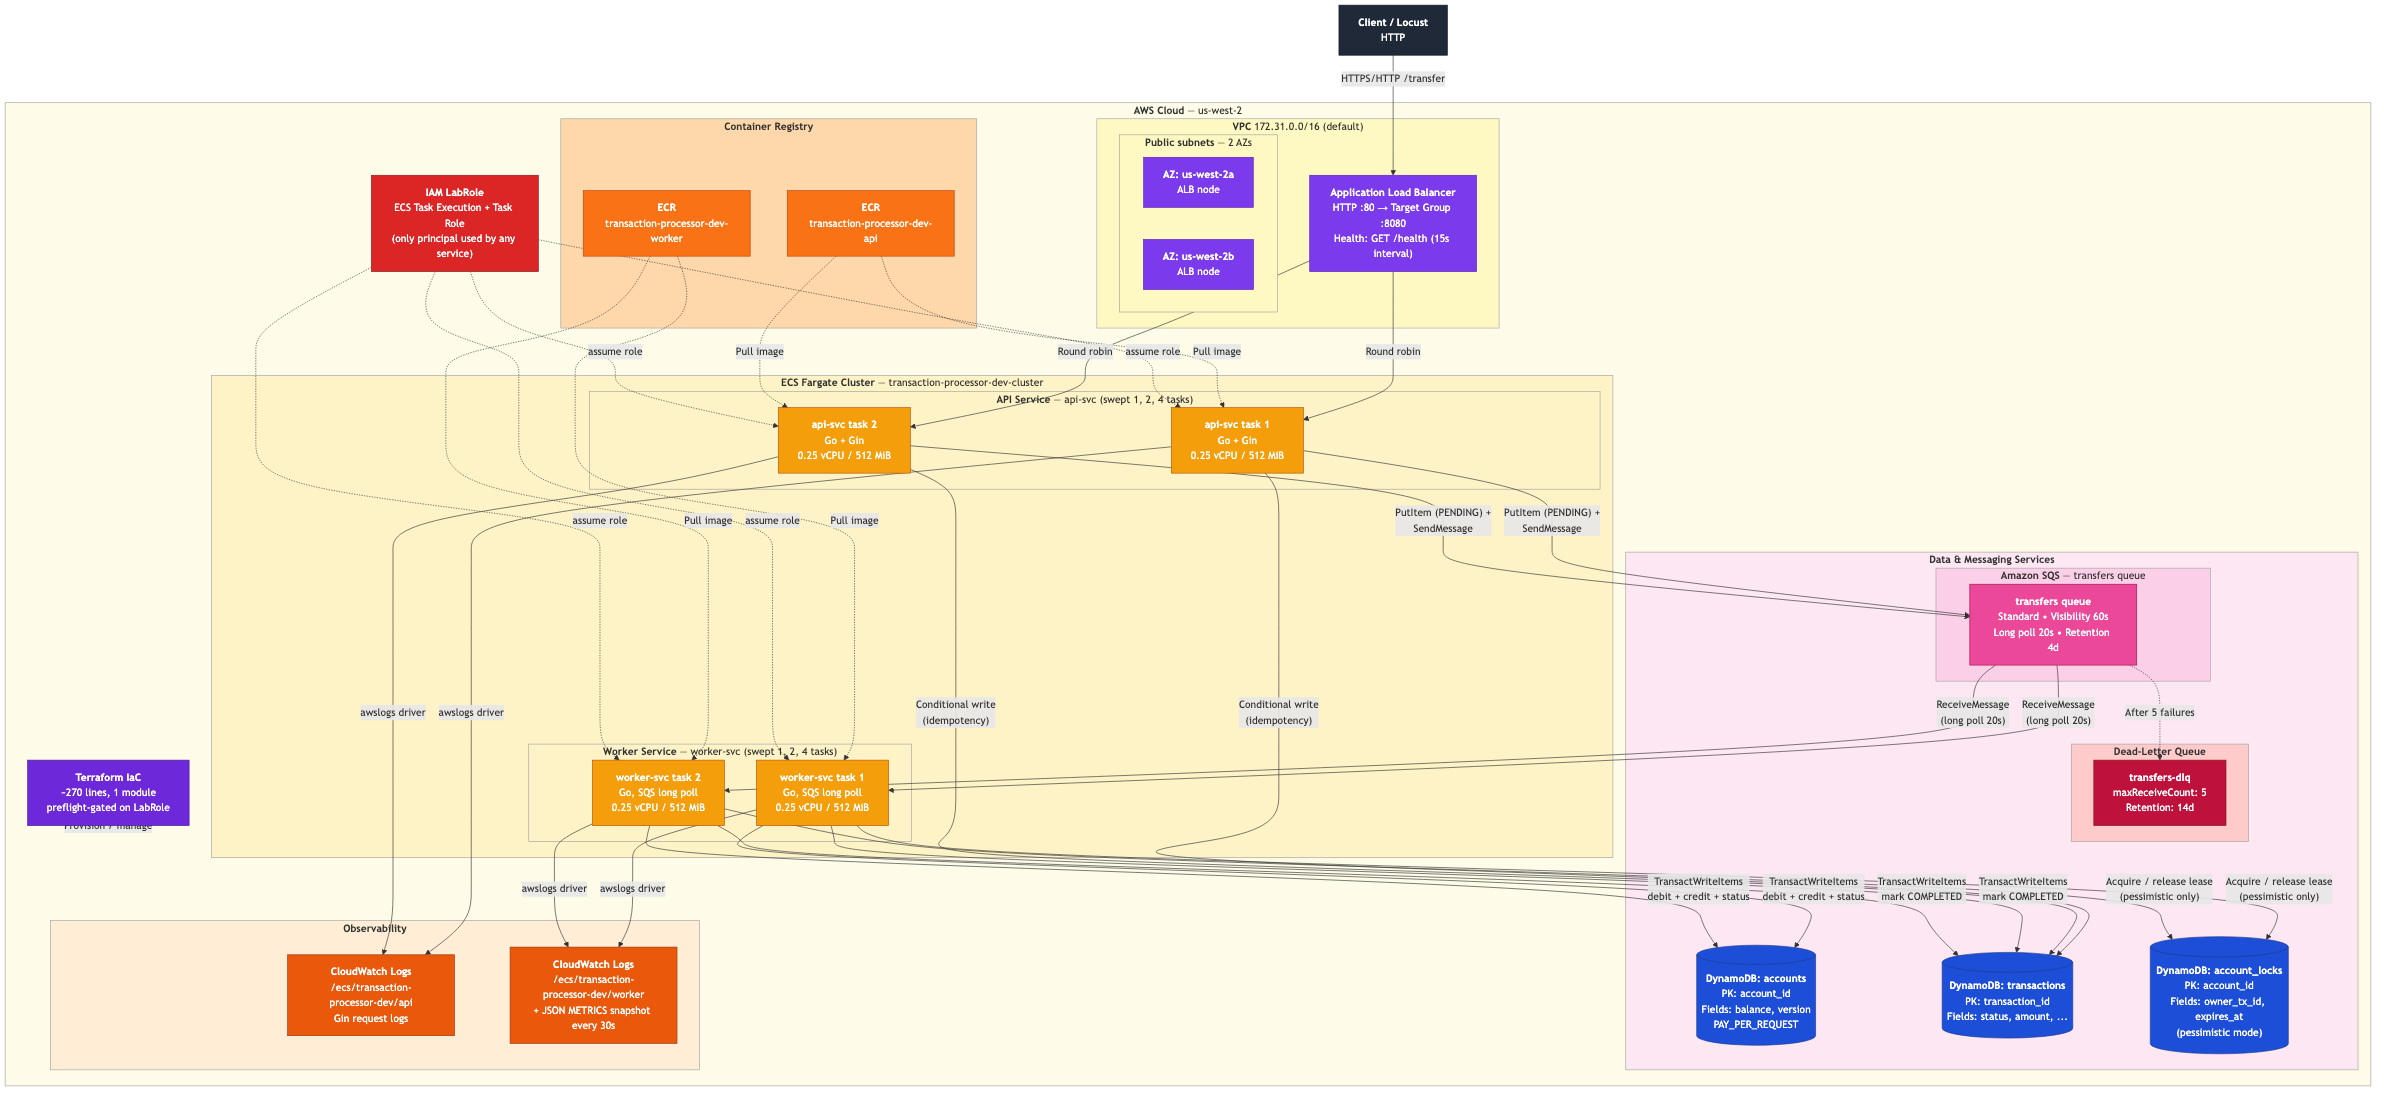
\includegraphics[width=\textwidth]{screenshots/arch-diagram.png}
\caption{Deployed architecture. Every arrow crosses an AWS service boundary; no component runs locally. Every ECS task runs under LabRole; the stack creates no IAM resources of its own. Terraform provisions everything inside the yellow AWS Cloud container.}
\label{fig:arch}
\end{figure}

The guiding decisions that came out of the architecture review were:
\begin{itemize}[leftmargin=*, itemsep=0.2em]
    \item \textbf{Asynchronous by default.} The API returns HTTP~202 the moment a transfer is accepted and enqueued. All balance mutation happens in the worker path. This lets us scale API and worker fleets independently and gives us a natural crash-safety story through queue redelivery.
    \item \textbf{One atomic commit per transfer.} Debit, credit, and transaction-status update are bundled into a single DynamoDB \texttt{TransactWriteItems} call. A mid-commit crash cannot leave money half-moved.
    \item \textbf{Cloud-only.} There would be no permanent local-compose workflow. All correctness and performance numbers in the final report would be collected against real AWS services (ALB, ECS Fargate, SQS, DynamoDB, CloudWatch).
    \item \textbf{LabRole everywhere.} The only IAM principal wired into ECS task execution and task roles is \texttt{LabRole}. Terraform creates no IAM resources.
\end{itemize}

%==============================================================
\section{Repository and Service Scaffolding}
%==============================================================

I laid out the repository so that the API service, the worker service, infrastructure, and test harnesses each live in their own top-level directory while sharing a single Go module. The resulting structure (after all work was completed) is shown in Listing~\ref{lst:layout}.

\begin{lstlisting}[caption={Repository layout.}, label={lst:layout}]
transaction-processor/
  api-svc/          # HTTP API: handlers, queue client, dynamo client, main.go
    Dockerfile
    handlers/       # /transfer (POST), /transfer/:id (GET), /health
    queue/          # SQS send wrapper
    db/             # DynamoDB accessors
    models/         # request/response and Transaction types
  worker-svc/       # Asynchronous transfer processor
    Dockerfile
    processor/      # optimistic + pessimistic paths
    queue/          # SQS receive/delete wrapper
    db/             # DynamoDB accessors, lock primitives
    metrics/        # prom-style counters + /metrics endpoint
  load-tests/       # Locust workloads + verify_balances.py
  scripts/          # seed, push-images, smoke, experiment runners, charts
  infra/            # Terraform stack (ECR, ECS, ALB, SQS, DynamoDB, CloudWatch)
  Makefile          # cloud-only targets, each preflight-gated
\end{lstlisting}

\subsection{API service skeleton}

I wrote the API service in Go using the Gin framework. The HTTP surface exposes three routes:

\begin{lstlisting}[language=Go, caption={Route registration in \texttt{api-svc/main.go}.}]
r := gin.Default()
r.GET("/health", handlers.HealthCheck)
r.POST("/transfer", h.PostTransfer)
r.GET("/transfer/:id", h.GetTransfer)
\end{lstlisting}

\texttt{/health} is the ALB's target-group health probe. \texttt{POST /transfer} accepts a JSON body with a client-supplied \texttt{transaction\_id} for idempotency; \texttt{GET /transfer/:id} lets the client poll the outcome. The \texttt{PostTransfer} handler validates the body, writes the pending record, and enqueues the message --- the three steps run sequentially against DynamoDB and SQS.

\subsection{Worker service skeleton}

The worker is a long-lived process that loops on \texttt{ReceiveMessage} with long polling. The processing function is isolated in \texttt{worker-svc/processor/} so the two locking strategies can swap behind a shared interface without touching the I/O code.

\begin{lstlisting}[language=Go, caption={Worker receive loop in \texttt{worker-svc/main.go}.}]
for {
    msgs, err := sqsClient.Receive(ctx)
    for _, msg := range msgs {
        var req models.TransferRequest
        json.Unmarshal([]byte(msg.Body), &req)
        if err := proc.Process(ctx, req); err != nil {
            // leave in queue for SQS to redeliver
            continue
        }
        sqsClient.Delete(ctx, msg.ReceiptHandle)
    }
}
\end{lstlisting}

The ``leave in queue on error'' semantics is deliberate: any error short of a terminal commit keeps the message visible for SQS to redeliver after the visibility timeout expires. Combined with the idempotency check at the top of \texttt{Process}, this gives the worker fleet at-least-once delivery without at-most-once complexity.

%==============================================================
\section{Core Transfer Workflow}
%==============================================================

This was joint work with my collaborator. My part of the implementation covered the API handler end-to-end and the overall orchestration in the worker; the DynamoDB conditional-write primitives were developed on the other track. Figure~\ref{fig:flow} shows the complete path of a single transfer.

\begin{figure}[H]
\centering
\begin{lstlisting}[caption={}, label={}, basicstyle=\ttfamily\small, frame=none]
  [API side]                           [Worker side]
  Client POST /transfer                Worker ReceiveMessage
           |                                    |
           v                                    v
  Validate + idempotency probe         GetTransaction status
           |                                    |
           v                                    v
  PutTransactionIfNotExists            status == PENDING ?
   (status = PENDING)                   |            |
           |                            v (no)       v (yes)
           v                      Delete msg     TransactWriteItems:
  SendMessage (SQS)  ---------->  return         debit + credit + COMPLETED
           |                                          |
           v                                          v
  Return HTTP 202                               Delete SQS message
\end{lstlisting}
\caption{End-to-end path of a single transfer across API and worker.}
\label{fig:flow}
\end{figure}

\subsection{API handler}

The \texttt{PostTransfer} handler is deliberately short. Its entire job is to accept the request, make a durable record of intent, enqueue it, and return. The actual money movement is left to the worker.

\begin{lstlisting}[language=Go, caption={Core of \texttt{PostTransfer}.}]
if req.TransactionID == "" || req.FromAccount == "" ||
    req.ToAccount == "" || req.Amount <= 0 {
    c.JSON(400, gin.H{"error": "invalid request"})
    return
}
if req.FromAccount == req.ToAccount {
    c.JSON(400, gin.H{"error": "from and to must differ"})
    return
}

existing, _ := h.db.GetTransaction(ctx, req.TransactionID)
if existing != nil {
    c.JSON(200, existing)  // idempotent replay
    return
}

created, _ := h.db.PutTransactionIfNotExists(ctx, tx)
if !created { /* lost the idempotency race, return existing */ }

h.queue.SendMessage(ctx, req)
c.JSON(202, models.TransferResponse{Status: "PENDING", ...})
\end{lstlisting}

\subsection{Worker orchestration}

On the worker side I wrote the top-level orchestration in \texttt{processor.Process}:

\begin{lstlisting}[language=Go, caption={Worker-side orchestration.}]
func (p *Processor) Process(ctx context.Context, req models.TransferRequest) error {
    tx, err := p.db.GetTransaction(ctx, req.TransactionID)
    if tx.Status == "COMPLETED" || tx.Status == "FAILED" {
        return nil  // redelivery short-circuit
    }
    return p.transfer(ctx, req)
}
\end{lstlisting}

The terminal-state short-circuit is what makes the worker safe against SQS redelivery. If a message is delivered twice, the second delivery sees a terminal status and returns without touching balances.

The \texttt{transfer} loop retries on retryable concurrency errors (conditional-check failures, transaction-cancelled reasons caused by version mismatches) with exponential backoff and a budget of three attempts. If all three attempts fail, the transaction is marked \texttt{FAILED} via a conditional update that only fires if the record is still \texttt{PENDING}.

%==============================================================
\section{SQS Integration}
%==============================================================

SQS was the component I owned end-to-end. It lives at two boundaries: the producer in the API service and the consumer in the worker service. Figure~\ref{fig:api-logs} shows the live API request log stream in CloudWatch during a Locust run: every \texttt{POST /transfer} returns HTTP~202 and is paired with an enqueue call.

\begin{figure}[H]
\centering
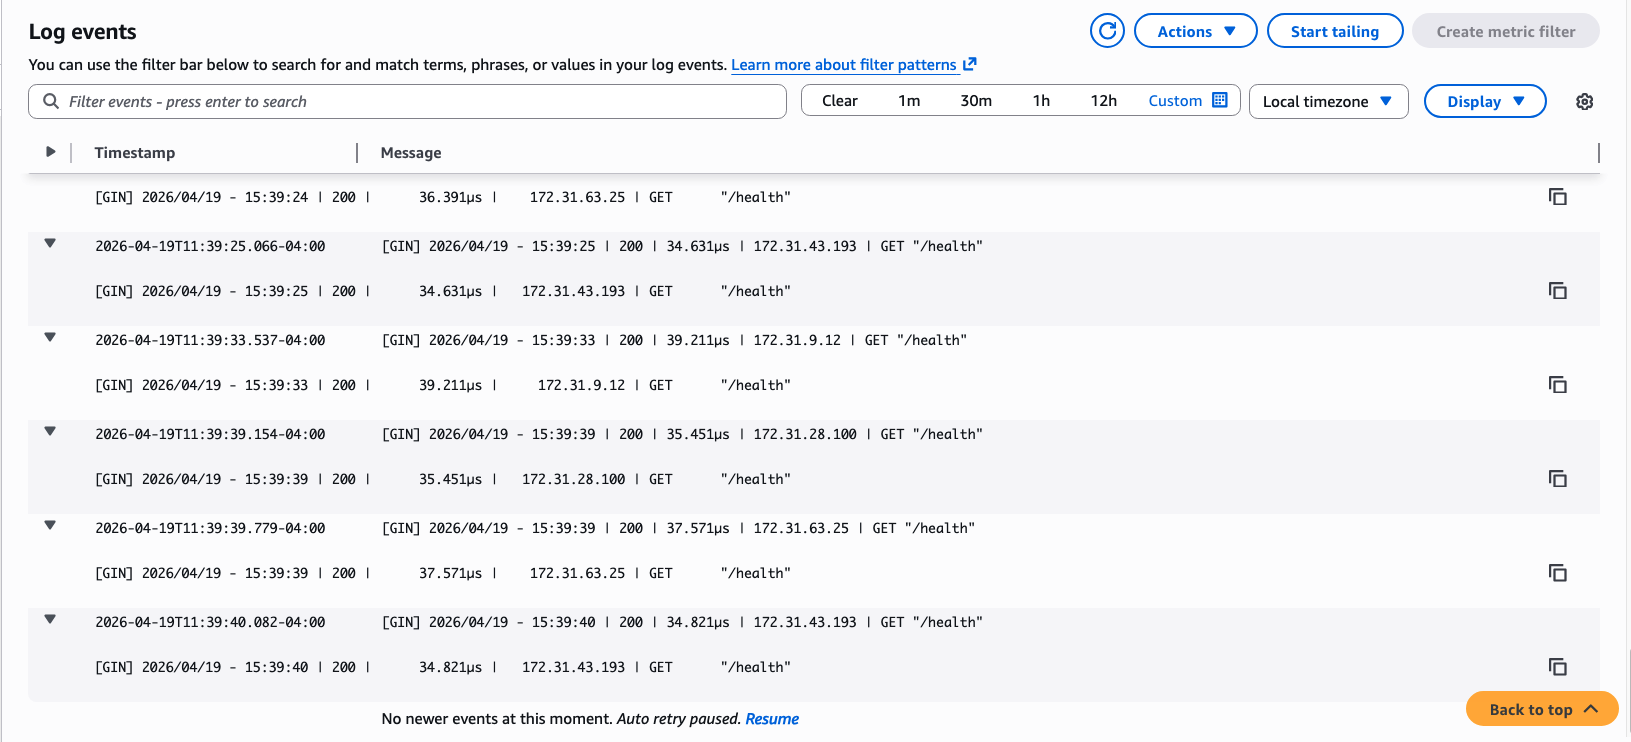
\includegraphics[width=0.95\textwidth]{screenshots/aws-cloudwatch-api-logs.png}
\caption{CloudWatch log stream for \texttt{api-svc} during a live load test. Every \texttt{POST /transfer} returns 202 and is followed by an SQS enqueue. Captured from the deployed stack in \texttt{us-west-2}.}
\label{fig:api-logs}
\end{figure}

\subsection{Producer side}

The API's producer uses the AWS SDK v2 client and serializes the transfer request as JSON into the message body:

\begin{lstlisting}[language=Go, caption={Producer wrapper (\texttt{api-svc/queue/sqs.go}).}]
func (c *SQSClient) SendMessage(ctx context.Context, req models.TransferRequest) error {
    body, _ := json.Marshal(req)
    _, err := c.client.SendMessage(ctx, &sqs.SendMessageInput{
        QueueUrl:    aws.String(c.queueURL),
        MessageBody: aws.String(string(body)),
    })
    return err
}
\end{lstlisting}

\subsection{Consumer side}

The worker uses a 20-second long poll so idle workers do not burn CPU on empty responses:

\begin{lstlisting}[language=Go, caption={Consumer wrapper (\texttt{worker-svc/queue/sqs.go}).}]
out, err := c.client.ReceiveMessage(ctx, &sqs.ReceiveMessageInput{
    QueueUrl:            aws.String(c.queueURL),
    MaxNumberOfMessages: 10,
    WaitTimeSeconds:     20,
})
\end{lstlisting}

\subsection{Reliability posture}

The queue is deployed with a dead-letter queue behind it. Any message that gets redelivered more than five times (due to repeated worker failures, poison payloads, or a persistently unavailable DynamoDB partition) is moved off the main queue automatically, so one bad message cannot stall the whole pipeline. The main queue's visibility timeout is set to 60~seconds --- long enough for a single transfer to commit comfortably, short enough that a crashed worker's in-flight messages come back to the queue quickly.

%==============================================================
\section{Containerization and Deployment Packaging}
%==============================================================

Both services are shipped as Docker images. I wrote multi-stage Dockerfiles that build a static Linux binary in a Go toolchain image and then copy only the binary into a minimal Alpine runtime image. Each image is on the order of 20~MiB.

\begin{lstlisting}[caption={\texttt{api-svc/Dockerfile} (the worker's is structurally identical).}]
FROM golang:1.22-alpine AS builder
WORKDIR /app
COPY go.mod go.sum ./
RUN go mod download
COPY . .
RUN go build -o /api-svc ./api-svc

FROM alpine:latest
WORKDIR /app
COPY --from=builder /api-svc .
EXPOSE 8080
CMD ["./api-svc"]
\end{lstlisting}

For cloud deployment I wrote \texttt{scripts/push\_images.sh}, which authenticates against ECR, builds both images for \texttt{linux/amd64}, and pushes them tagged \texttt{:latest}. The cross-platform build is essential because my development laptop is Apple Silicon; a naive \texttt{docker build} produces ARM64 images that Fargate's default \texttt{linux/amd64} runtime cannot pull. The script uses \texttt{docker buildx} with an explicit \texttt{--platform linux/amd64} so the manifest always matches Fargate's runtime (Section~\ref{sec:obstacles}).

Figure~\ref{fig:ecr} shows both images pushed to ECR, tagged \texttt{latest}, with their digests recorded.

\begin{figure}[H]
\centering
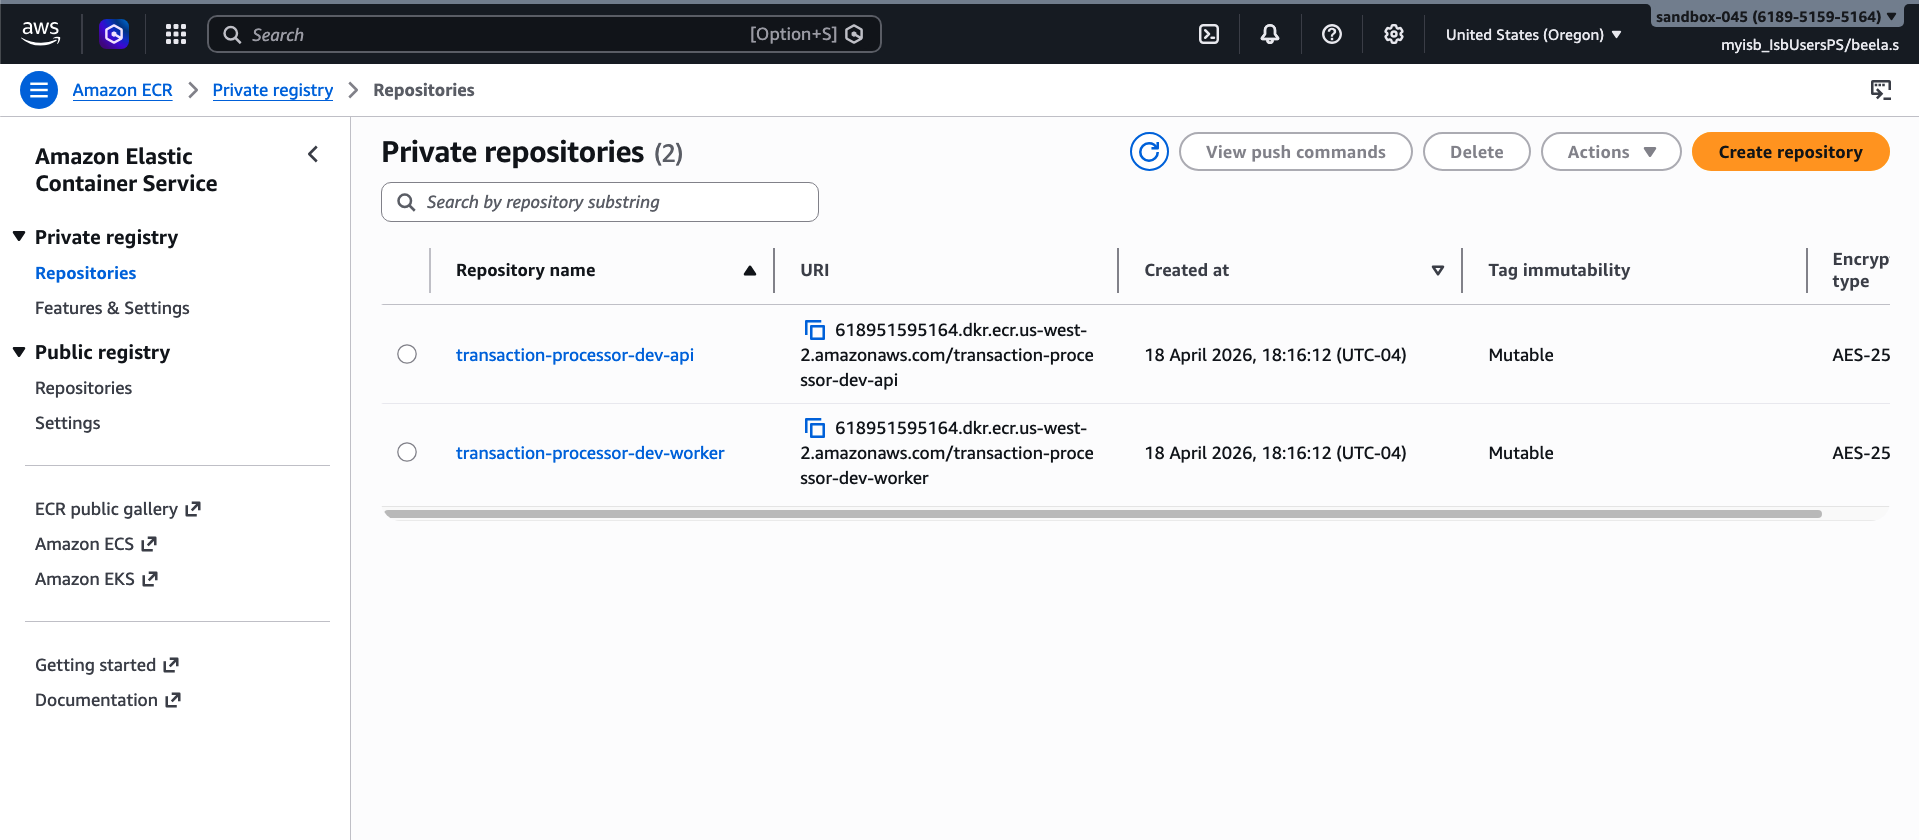
\includegraphics[width=0.95\textwidth]{screenshots/aws-ecr-images.png}
\caption{ECR repositories \texttt{transaction-processor-dev-api} and \texttt{transaction-processor-dev-worker} after \texttt{make push-images}. Both images are \texttt{linux/amd64} manifests.}
\label{fig:ecr}
\end{figure}

%==============================================================
\section{Cloud Smoke Testing}
%==============================================================

The smoke test proves the entire deployed pipeline end-to-end: ALB $\rightarrow$ API $\rightarrow$ DynamoDB (pending) $\rightarrow$ SQS $\rightarrow$ worker $\rightarrow$ DynamoDB (completed). I wrote \texttt{scripts/smoke\_test.sh} (joint with my collaborator for the final cloud variant) to submit a single transfer against the ALB and poll the status endpoint until the transaction reaches \texttt{COMPLETED} or \texttt{FAILED}.

\begin{lstlisting}[caption={Smoke output against the deployed stack.}]
Health check passed for http://transaction-processor-dev-alb-...us-west-2.elb.amazonaws.com
Submitted transfer 9fd50eb0-d504-4a1a-acd1-c600419d0f52; polling for completion
{"transaction_id":"9fd50eb0-...","status":"COMPLETED","amount":10,
 "from_account":"account-0","to_account":"account-1","created_at":"2026-04-18T23:31:22Z"}
\end{lstlisting}

The smoke test is the first gate any cloud change must pass. It is also wrapped behind \texttt{make cloud-smoke}, which is itself gated by the LabRole preflight check so it cannot run under the wrong credentials.

Figures~\ref{fig:ecs-cluster}, \ref{fig:ecs-tasks}, and~\ref{fig:alb-healthy} are the AWS-side confirmation that the deployed stack is live: the ECS cluster shows both services running their desired task counts, the Fargate task list shows the actual running tasks on AWS, and the ALB target group reports healthy targets.

\begin{figure}[H]
\centering
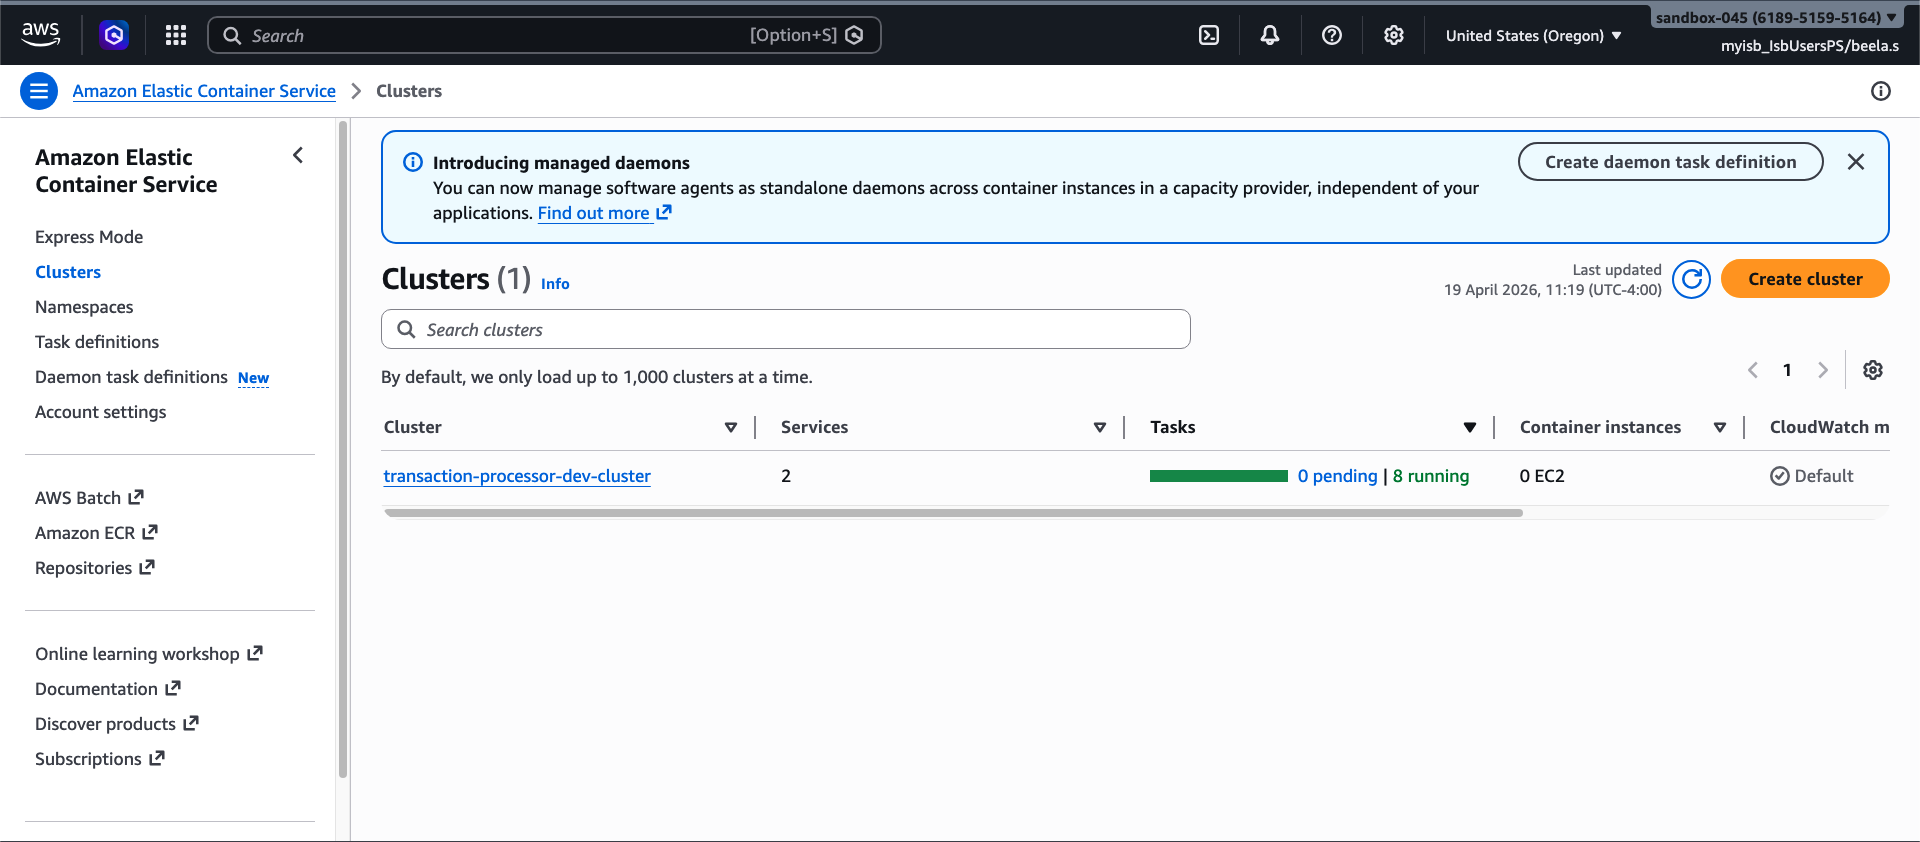
\includegraphics[width=0.95\textwidth]{screenshots/aws-ecs-cluster.png}
\caption{ECS cluster \texttt{transaction-processor-dev-cluster} with both \texttt{api} and \texttt{worker} services active.}
\label{fig:ecs-cluster}
\end{figure}

\begin{figure}[H]
\centering
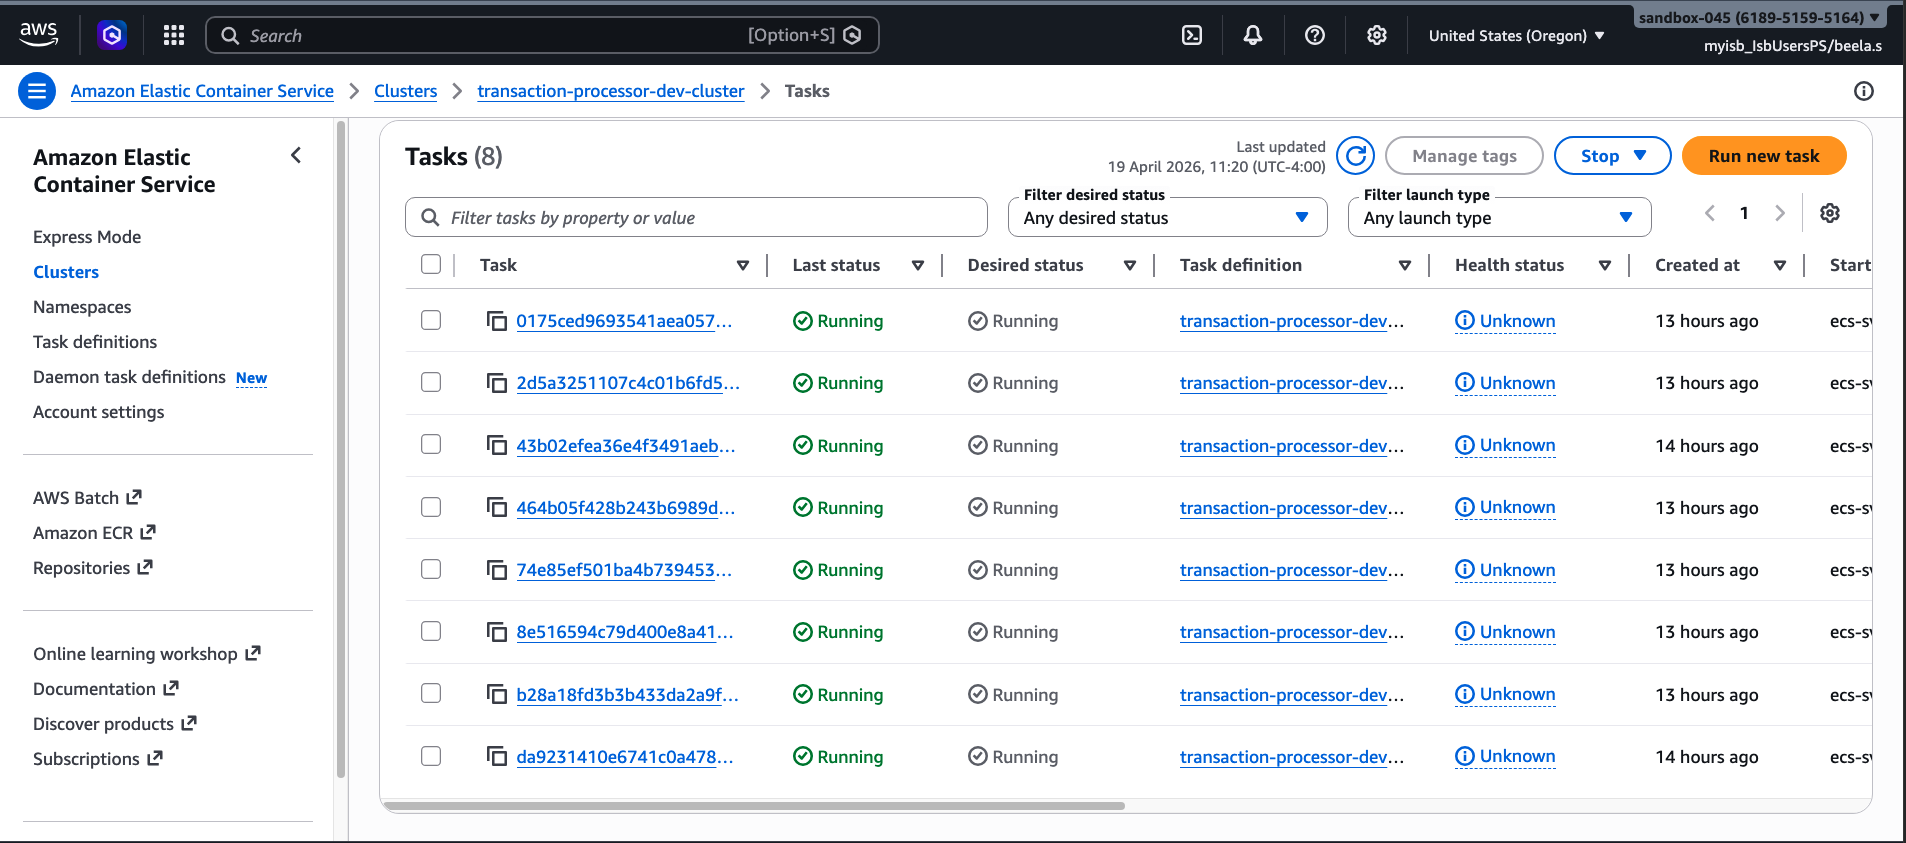
\includegraphics[width=0.95\textwidth]{screenshots/aws-ecs-tasks-running.png}
\caption{Running Fargate tasks for the worker service. Each task carries \texttt{LabRole} as its task role.}
\label{fig:ecs-tasks}
\end{figure}

\begin{figure}[H]
\centering
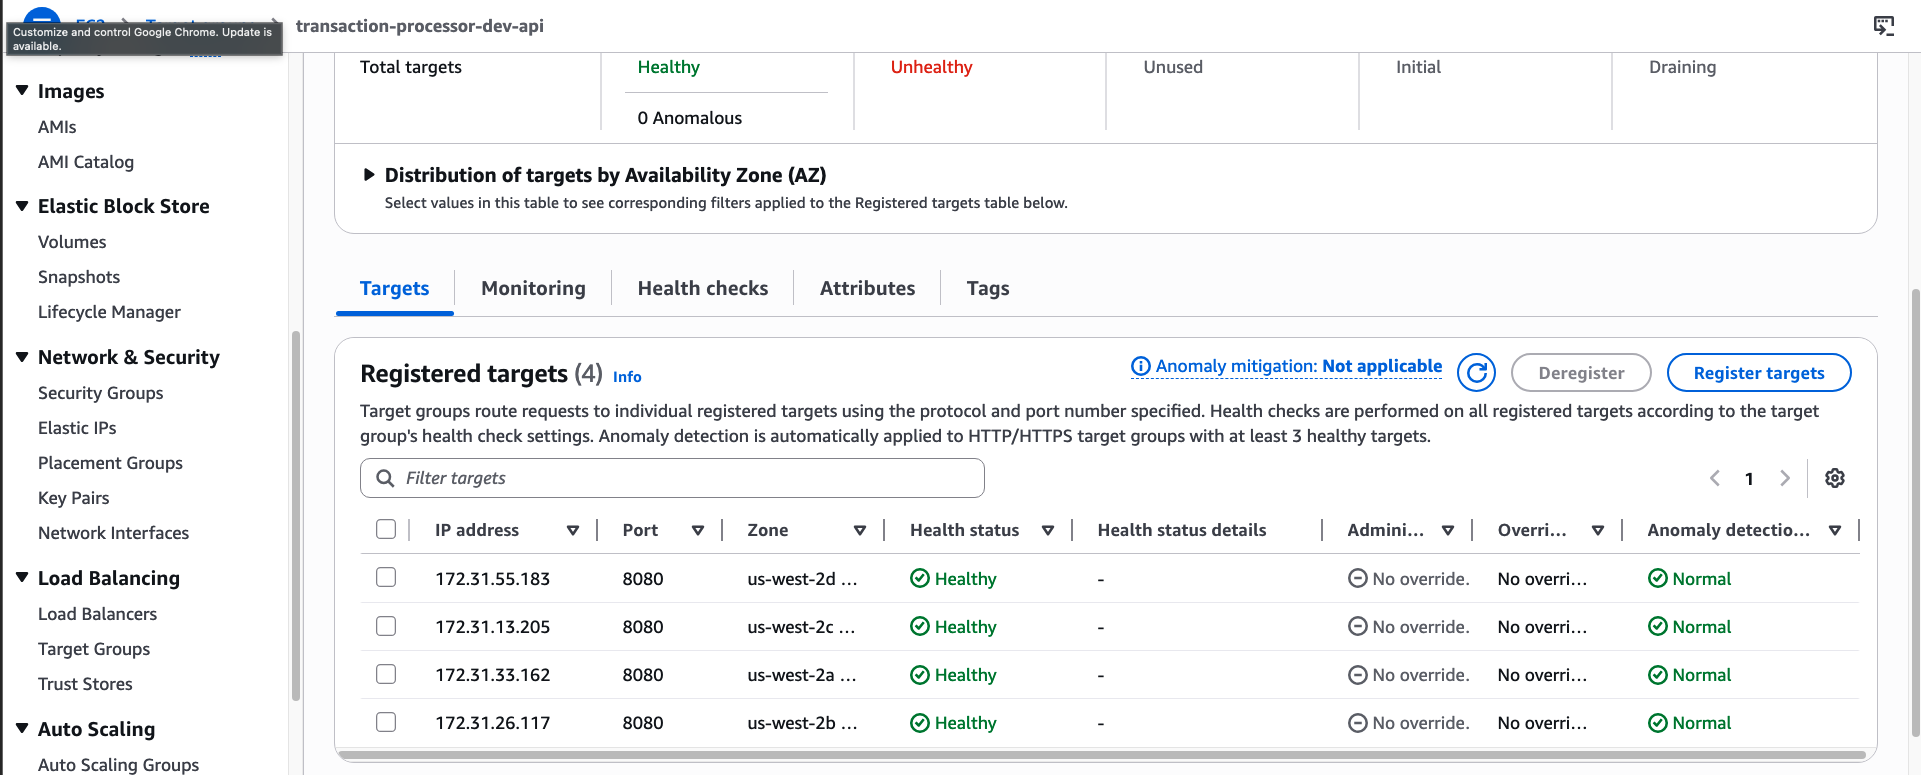
\includegraphics[width=0.95\textwidth]{screenshots/aws-alb-targets-healthy.png}
\caption{ALB target group showing the API task healthy --- the \texttt{/health} probe is succeeding.}
\label{fig:alb-healthy}
\end{figure}

%==============================================================
\section{Load Testing Framework}
%==============================================================

I built the load-testing harness in Locust (Python). The harness supports two user classes that map directly to the experiments in the plan:

\begin{description}[leftmargin=*]
    \item[\texttt{TransferUser}] Picks two distinct accounts at random from a seeded pool of 100, sends a transfer with a random amount in \$1.00--\$100.00. Models mixed traffic.
    \item[\texttt{HotAccountUser}] All senders are \texttt{hot-account-001}. Used to create deliberate contention on a single account for the optimistic-vs-pessimistic comparison.
\end{description}

\begin{lstlisting}[language=Python, caption={Core of \texttt{locustfile.py}.}]
class HotAccountUser(HttpUser):
    wait_time = between(0.05, 0.2)

    @task
    def hot_transfer(self):
        to_acct = random.choice([a for a in _ACCOUNT_IDS if a != "hot-account-001"])
        payload = {
            "transaction_id": str(uuid.uuid4()),
            "from_account": "hot-account-001",
            "to_account": to_acct,
            "amount": 1.0,
        }
        resp = self.client.post("/transfer", json=payload, ...)
\end{lstlisting}

The harness exports CSV statistics (aggregated plus history), a rendered HTML report, and explicit failure files that become part of every experiment's artifact bundle. The Makefile exposes two cloud-targeted load profiles (\texttt{cloud-test-load} and \texttt{cloud-test-load-hot}) that point Locust at the ALB address from the Terraform outputs rather than any local endpoint.

Figures~\ref{fig:locust-transfer-25-charts} and~\ref{fig:locust-transfer-25-stats} show the Locust web UI during a baseline \texttt{TransferUser} run at 25 users against the deployed ALB. The live charts demonstrate requests-per-second, response-time percentiles, and user ramp-up in real time; the statistics tab breaks the request counts down by endpoint and percentile.

\begin{figure}[H]
\centering
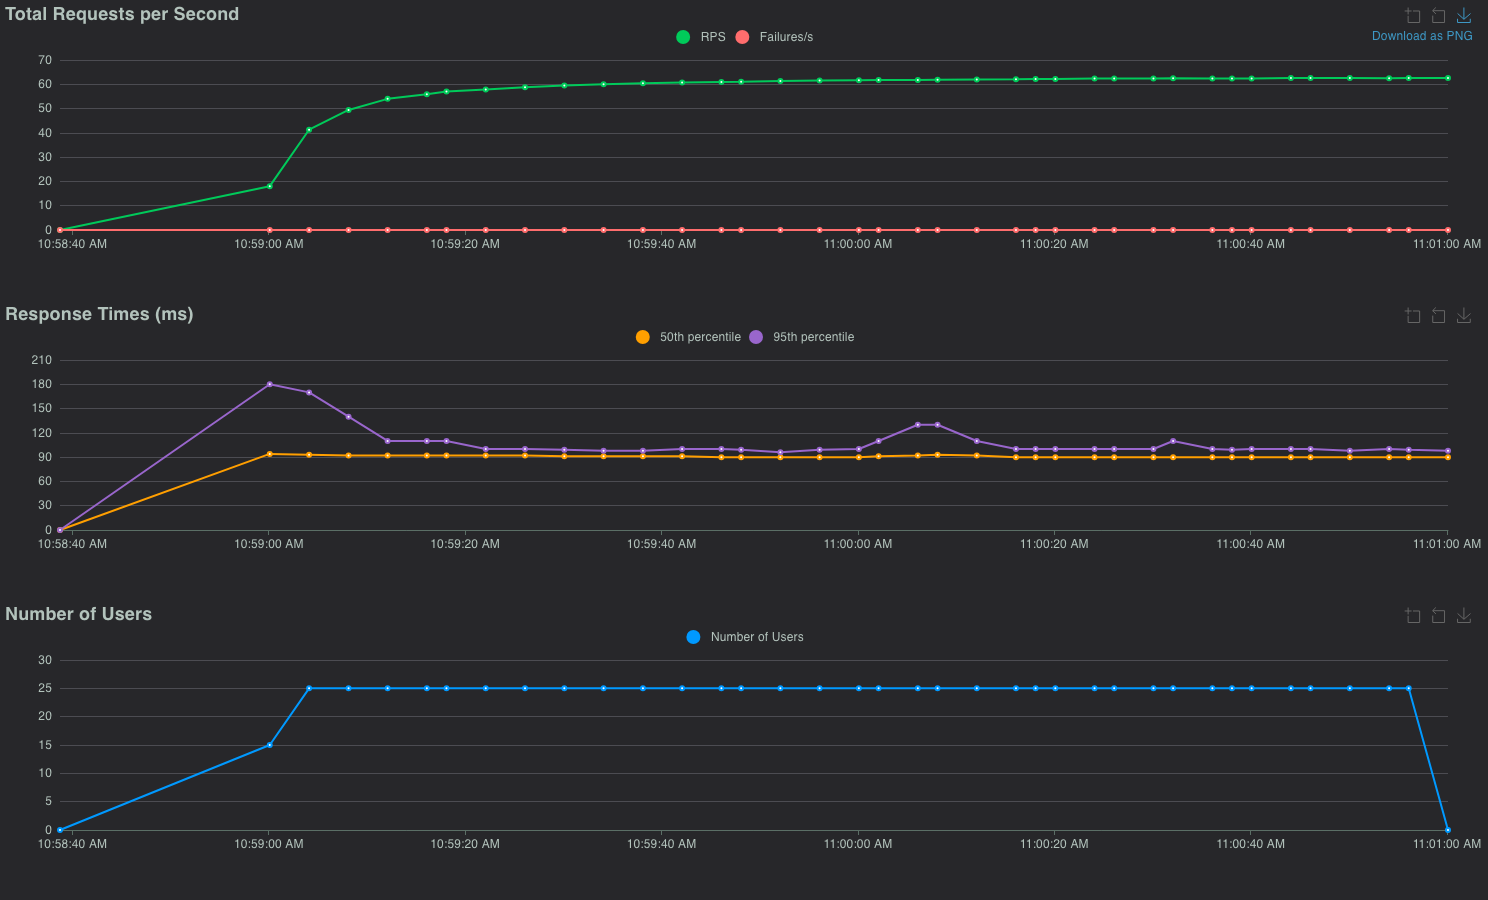
\includegraphics[width=0.95\textwidth]{screenshots/locust-transfer-25u-charts.png}
\caption{Locust web UI --- Charts tab during a 25-user \texttt{TransferUser} run against the ALB.}
\label{fig:locust-transfer-25-charts}
\end{figure}

\begin{figure}[H]
\centering
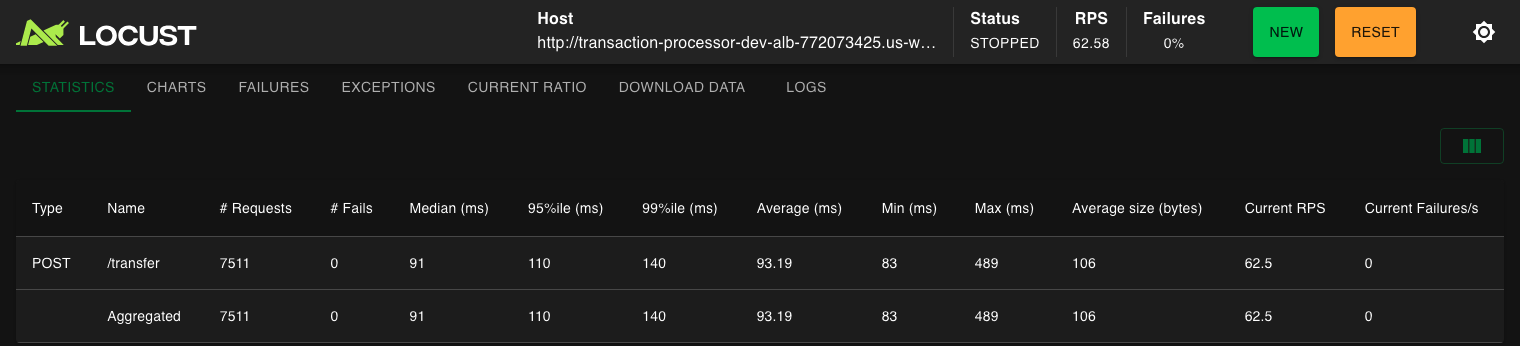
\includegraphics[width=0.95\textwidth]{screenshots/locust-transfer-25u-stats.png}
\caption{Locust web UI --- Statistics tab for the same run, showing per-endpoint request counts and percentile response times.}
\label{fig:locust-transfer-25-stats}
\end{figure}

%==============================================================
\section{Experiment~1 --- Concurrent Transfer Storm}
%==============================================================

\subsection{Objective}
Drive heavy contention against a single sender account and confirm that (1) the system continues to serve requests, (2) the balance invariant is preserved, and (3) we can measure the tail-latency cost of the contention.

\subsection{Setup}
\begin{itemize}[leftmargin=*, itemsep=0.2em]
    \item Workload: \texttt{HotAccountUser}, 50 virtual users, 5-minute headless run.
    \item Deployment: 1 API task, 1 worker task, optimistic locking mode.
    \item ALB URL from the Terraform outputs; all traffic crosses the public ALB.
\end{itemize}

\subsection{Results}

The aggregated Locust export is shown in Table~\ref{tab:exp1}.

\begin{table}[H]
\centering
\caption{Experiment~1 aggregated Locust statistics.}
\label{tab:exp1}
\begin{tabular}{lrrrrrr}
\toprule
Metric & Requests & Failures & Median & p95 & p99 & Req/s \\
\midrule
/transfer [hot] & 34{,}550 & 0 & 290~ms & 530~ms & 640~ms & 115.6 \\
\bottomrule
\end{tabular}
\end{table}

Every request succeeded at the HTTP layer. The p95 of 530~ms is dominated by the fact that every single transfer contends on the same sender's \texttt{version} attribute in DynamoDB: the optimistic path in the worker must retry whenever two workers read the same version and race to write it back. At this workload the worker fleet absorbs all of that retry cost without the API seeing any failures.

After the run, \texttt{verify\_balances.py} (owned by my collaborator) reported:

\begin{lstlisting}
Accounts scanned : 101
Expected total   : 1010000.00
Actual total     : 1010000.00
Difference       : 0.00
All balances correct.
\end{lstlisting}

No money was created or destroyed. This is the correctness invariant the whole project exists to uphold, and Experiment~1 is the first place it was exercised at realistic volume.

Figures~\ref{fig:locust-hot-50-charts} and~\ref{fig:locust-hot-50-stats} capture the Locust web UI during the hot-account storm. The charts show a sustained request-per-second plateau and a p95 response time that stays well inside the second the entire run. Figure~\ref{fig:sqs-inflight} is the AWS-side confirmation: the SQS queue's \texttt{ApproximateNumberOfMessagesNotVisible} graph spikes during the run, proving the queue is actually buffering in-flight transfers rather than being a silent pipe. Figure~\ref{fig:ddb-accounts} shows the \texttt{accounts} DynamoDB table's Monitor tab with consumed write-capacity spiking throughout the run window.

\begin{figure}[H]
\centering
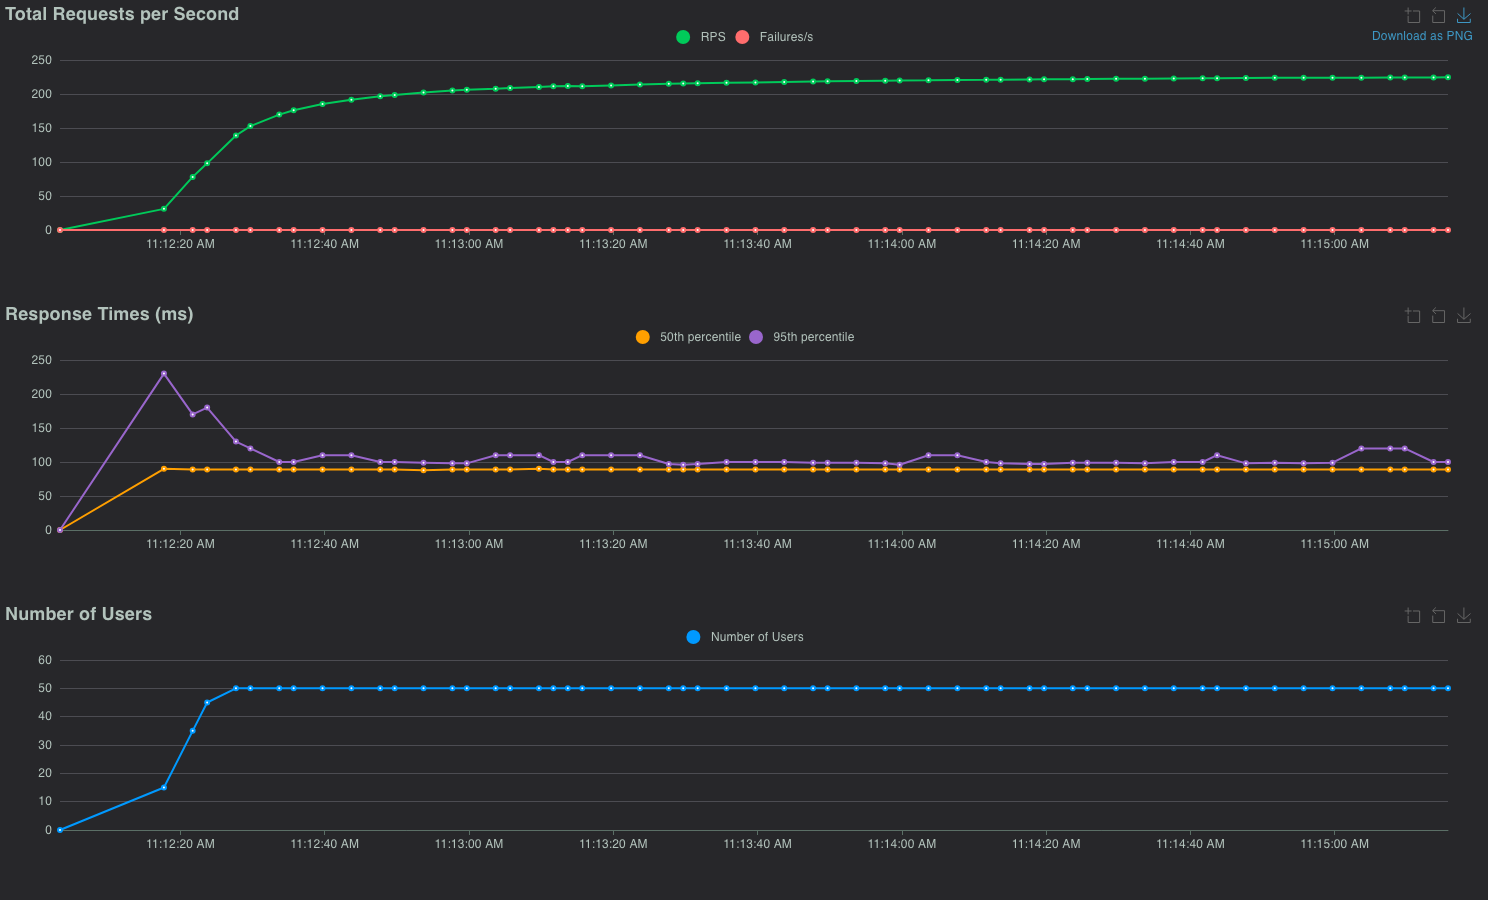
\includegraphics[width=0.95\textwidth]{screenshots/locust-hot-50u-charts.png}
\caption{Experiment~1 --- Locust Charts tab at 50 virtual \texttt{HotAccountUser} users.}
\label{fig:locust-hot-50-charts}
\end{figure}

\begin{figure}[H]
\centering
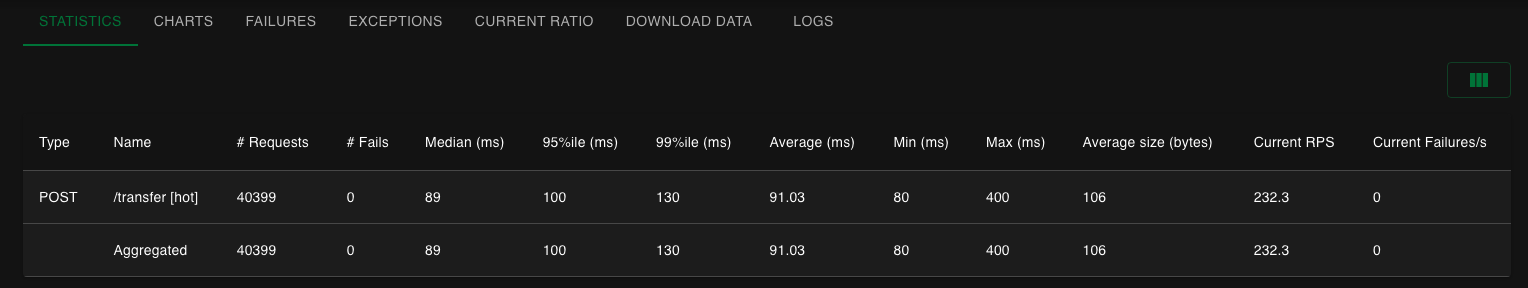
\includegraphics[width=0.95\textwidth]{screenshots/locust-hot-50u-stats.png}
\caption{Experiment~1 --- Locust Statistics tab. 34{,}550 transfers succeeded with zero failures.}
\label{fig:locust-hot-50-stats}
\end{figure}

\begin{figure}[H]
\centering
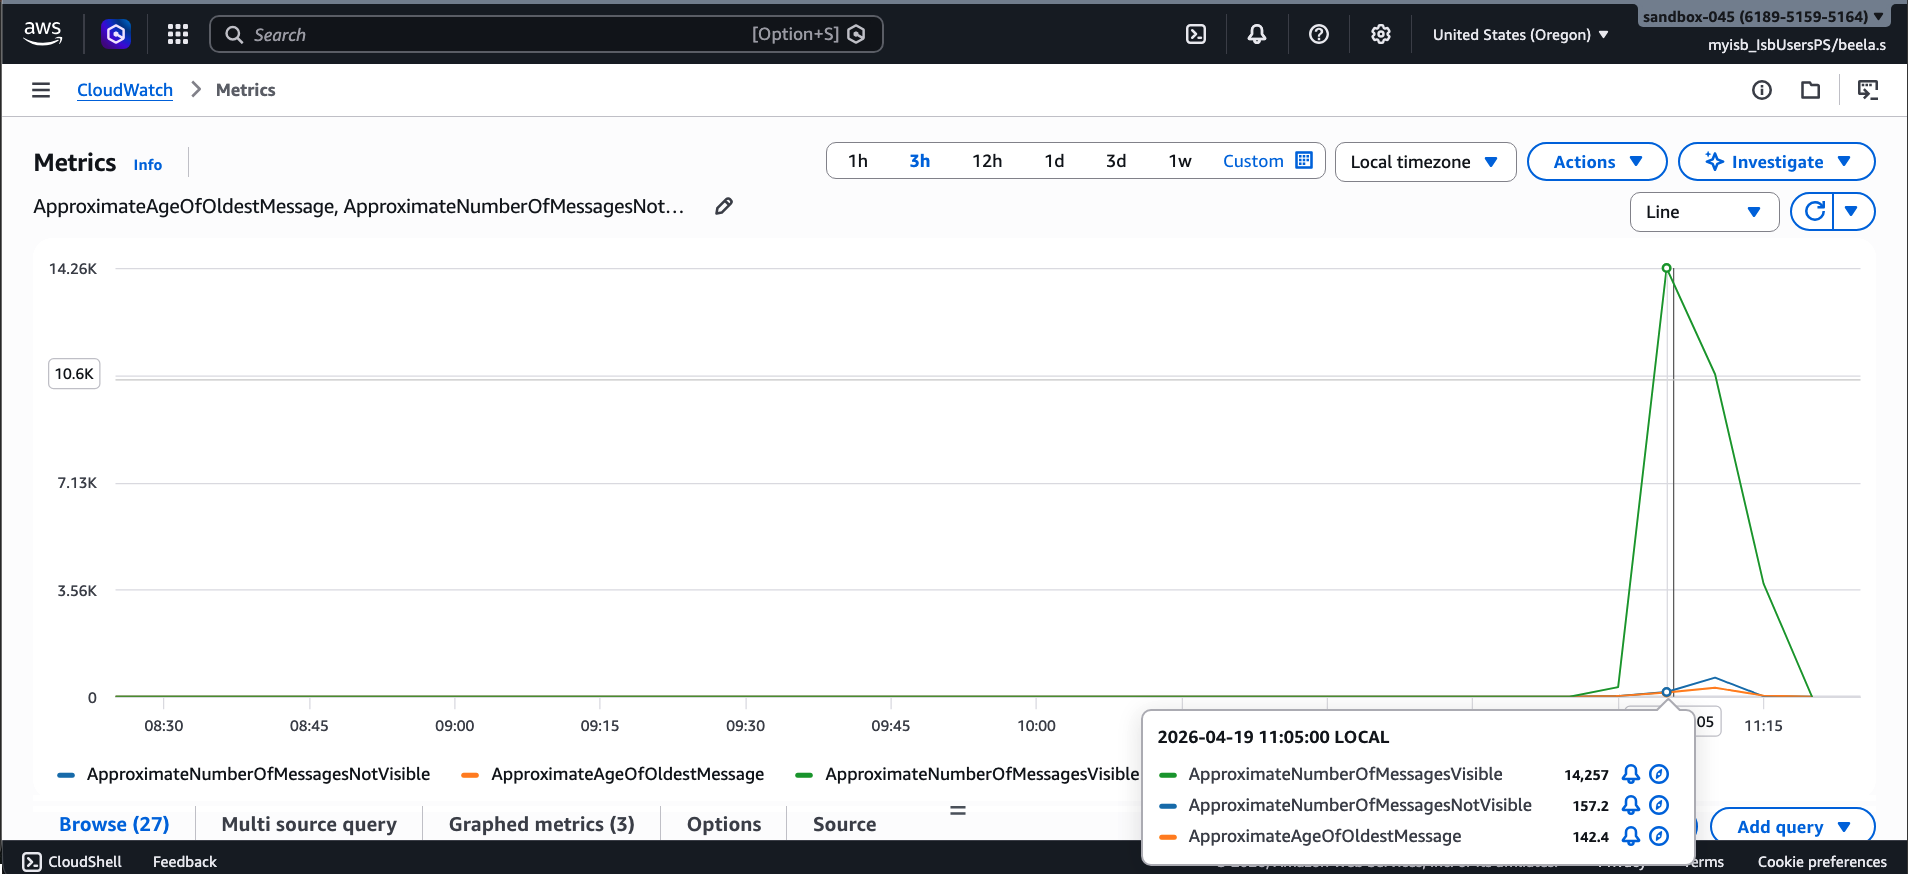
\includegraphics[width=0.95\textwidth]{screenshots/aws-sqs-messages-inflight.png}
\caption{SQS Monitoring tab during the run. In-flight message counts climb as workers pick up the load, then drain cleanly afterward.}
\label{fig:sqs-inflight}
\end{figure}

\begin{figure}[H]
\centering
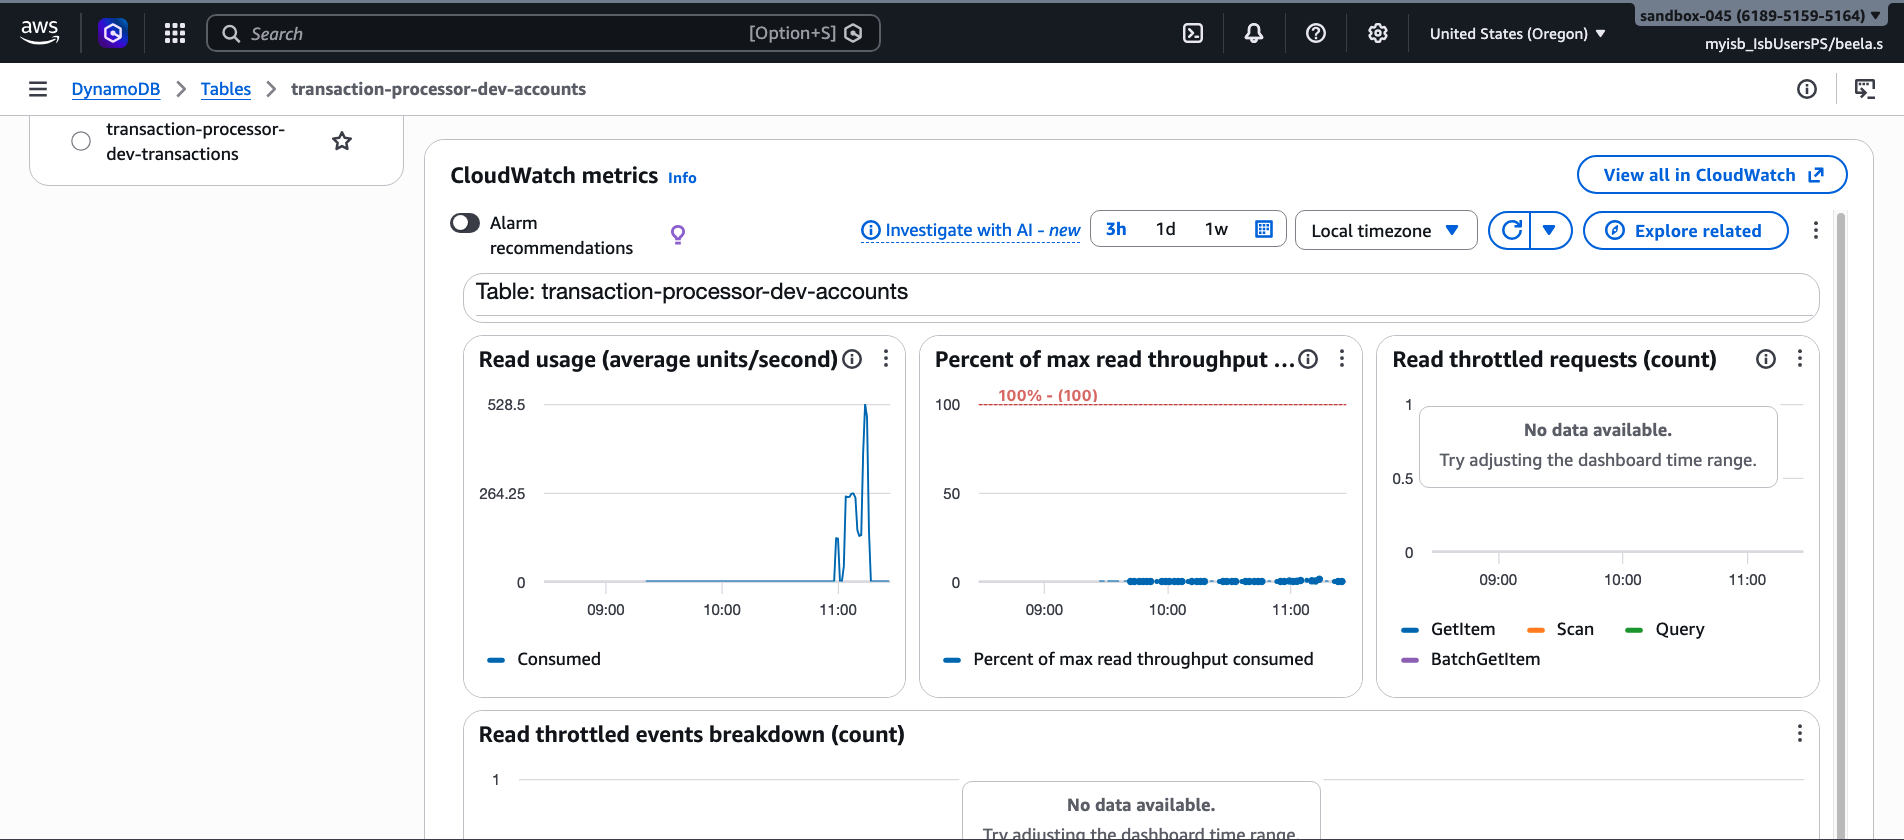
\includegraphics[width=0.95\textwidth]{screenshots/aws-dynamodb-accounts-monitor.png}
\caption{DynamoDB \texttt{accounts} table Monitor tab during the same run. Consumed write capacity tracks the Locust throughput exactly.}
\label{fig:ddb-accounts}
\end{figure}

%==============================================================
\section{Experiment~3 --- Optimistic vs. Pessimistic (Cloud)}
%==============================================================

\subsection{Objective}
Compare the two concurrency-control strategies head-to-head on AWS, at two contention levels, using the same hot-account workload. My collaborator built the pessimistic locking path; my contribution was the experiment harness, the measurement methodology, the metrics plumbing through CloudWatch, and the analysis of the resulting numbers.

\subsection{Harness}
I wrote \texttt{scripts/compare\_locking\_modes.sh}, a cloud-targeted runner that:
\begin{enumerate}[leftmargin=*, itemsep=0.2em]
    \item Flips the worker's \texttt{LOCKING\_MODE} environment variable via \texttt{terraform apply -var}.
    \item Waits for the ECS worker service to stabilize on the new task definition revision.
    \item Purges SQS and reseeds accounts so each run starts from an identical state.
    \item Executes a headless Locust run against the ALB.
    \item Waits for the queue to fully drain (both \texttt{ApproximateNumberOfMessages} and \texttt{ApproximateNumberOfMessagesNotVisible} reach zero).
    \item Snapshots cumulative worker counters from CloudWatch Logs.
    \item Verifies balances on the cloud accounts table.
\end{enumerate}

\subsection{Results}

\begin{table}[H]
\centering
\caption{Experiment~3 cloud numbers. Two worker replicas, hot-account workload, 2-minute runs.}
\label{tab:exp3}
\begin{tabular}{lrrrrrrr}
\toprule
Mode & Users & Requests & Failures & Avg ms & p95 ms & p99 ms & Req/s \\
\midrule
Optimistic  & 25 & 12{,}987 & 0 & 98.14  & 130 & 180 & 108.84 \\
Optimistic  & 50 & 13{,}574 & 0 & 296.21 & 540 & 650 & 113.78 \\
Pessimistic & 25 & 13{,}256 & 0 & 94.77  & 120 & 140 & 111.15 \\
Pessimistic & 50 & 13{,}693 & 0 & 292.19 & 540 & 660 & 114.52 \\
\bottomrule
\end{tabular}
\end{table}

\begin{figure}[H]
\centering
\begin{subfigure}[b]{0.48\textwidth}
    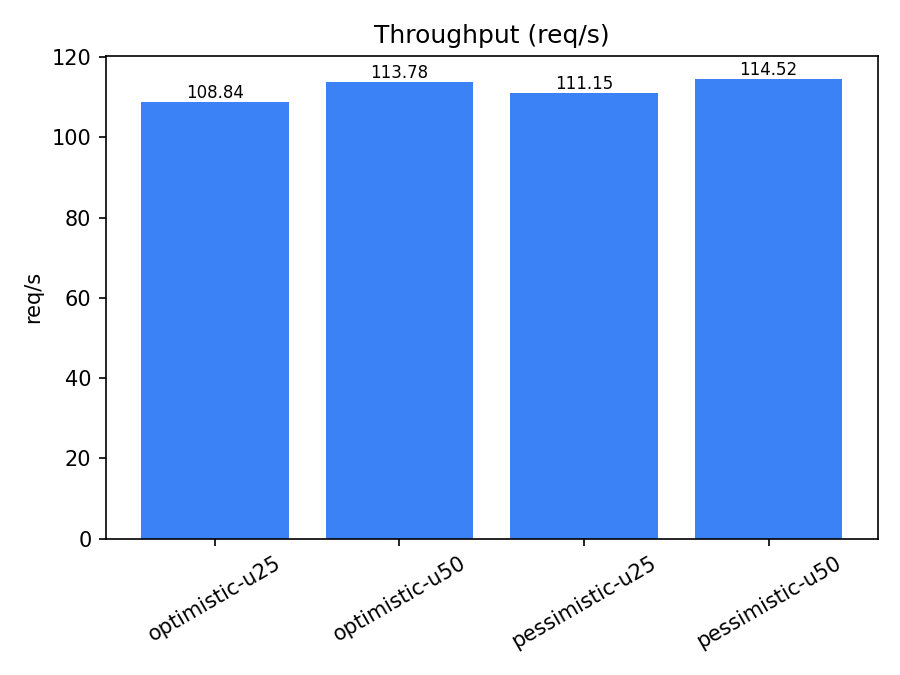
\includegraphics[width=\textwidth]{experiments/20260418-200951/throughput.png}
    \caption{Throughput by mode and user count.}
\end{subfigure}
\hfill
\begin{subfigure}[b]{0.48\textwidth}
    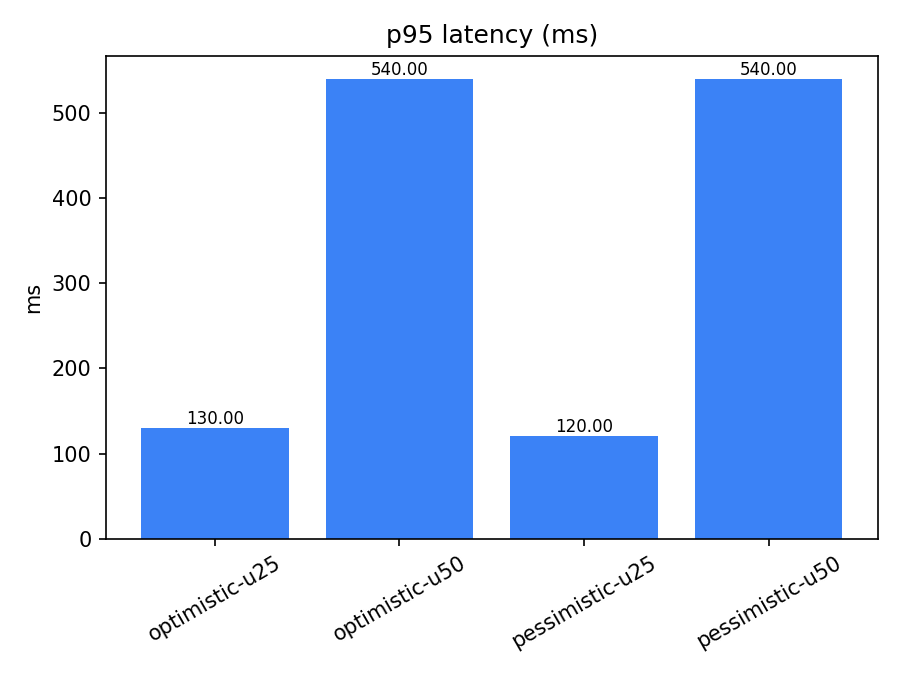
\includegraphics[width=\textwidth]{experiments/20260418-200951/p95_latency.png}
    \caption{p95 latency by mode and user count.}
\end{subfigure}
\caption{Experiment~3 aggregate throughput and latency.}
\label{fig:exp3a}
\end{figure}

\begin{figure}[H]
\centering
\begin{subfigure}[b]{0.48\textwidth}
    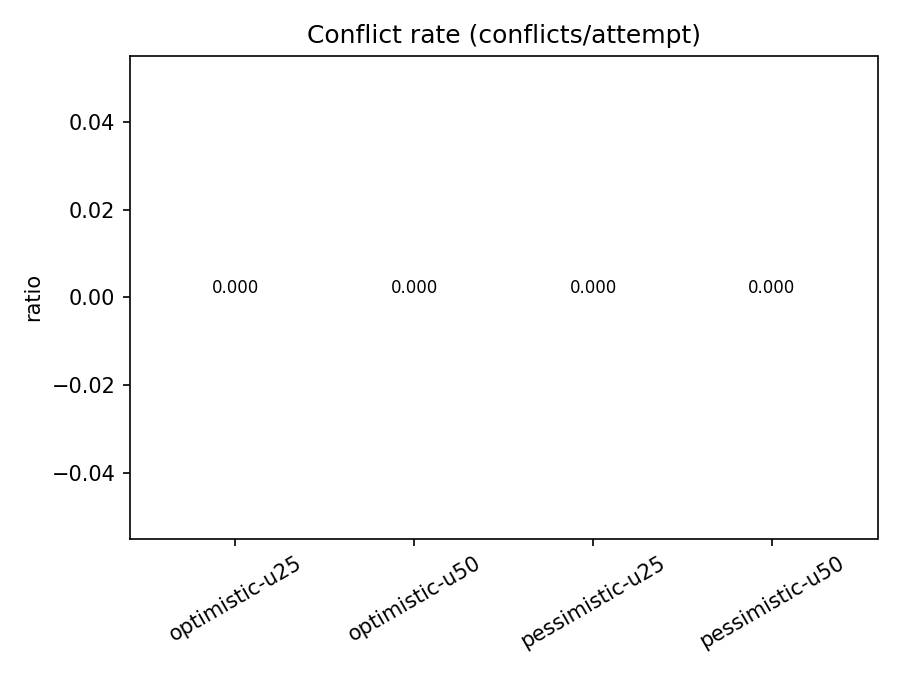
\includegraphics[width=\textwidth]{experiments/20260418-200951/conflict_rate.png}
    \caption{Conflict rate (conflicts per attempt).}
\end{subfigure}
\hfill
\begin{subfigure}[b]{0.48\textwidth}
    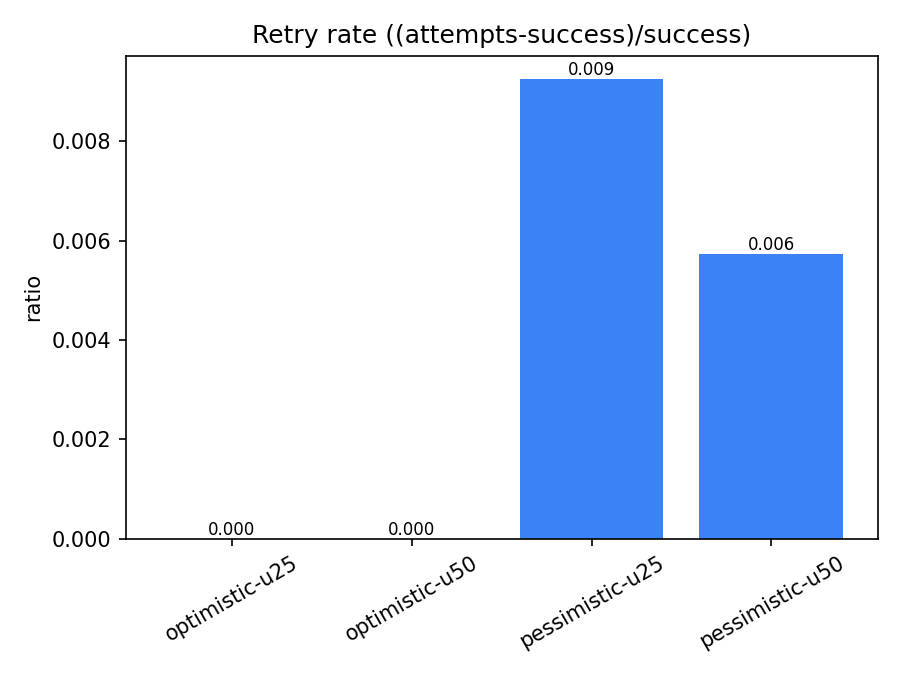
\includegraphics[width=\textwidth]{experiments/20260418-200951/retry_rate.png}
    \caption{Retry rate ((attempts $-$ success) / success).}
\end{subfigure}
\caption{Experiment~3 worker-side conflict and retry behavior from CloudWatch counter snapshots.}
\label{fig:exp3b}
\end{figure}

\subsection{Discussion}

The two modes produced statistically indistinguishable throughput (108--115~req/s across all four runs). That surprised me initially; I expected pessimistic to lose ground because it pays for an explicit lock write on each transfer. The reason they tie is that at this workload the bottleneck is the single-partition write rate on the hot account itself, not the locking mechanism: both modes must serialize writes to that partition, and both eventually do.

Where the modes diverge is in the tail:
\begin{itemize}[leftmargin=*, itemsep=0.2em]
    \item At 25 users, pessimistic's p95 is 120~ms vs. optimistic's 130~ms. Optimistic pays a 100~ms, then 200~ms, then 400~ms backoff on each conflict; pessimistic does not retry, so its latency is tighter.
    \item At 50 users, both modes plateau at p95 = 540~ms. The queue depth and SQS round-trip time dominate any per-request difference.
    \item Conflict and retry rates (Figure~\ref{fig:exp3b}) are effectively zero for pessimistic and non-trivial for optimistic, as expected from first principles.
\end{itemize}

The headline lesson: optimistic is the right default for low-contention workloads, but it does not scale gracefully as contention grows because every conflict costs a full backoff cycle. Pessimistic pays a fixed small tax up front that flattens the tail.

Figures~\ref{fig:locust-hot-25-charts} and~\ref{fig:locust-hot-25-stats} show the Locust-side view of the 25-user hot-account run that feeds Table~\ref{tab:exp3}. Figure~\ref{fig:ddb-cond-fails} is arguably the most informative chart in the experiment: the DynamoDB \texttt{ConditionalCheckFailedRequests} metric, taken over the window when the locking mode was flipped from optimistic to pessimistic. The metric rises under optimistic traffic (every retry is a conditional-check failure that DynamoDB observes) and drops to effectively zero once the pessimistic path is active, which lines up with the zero conflict rate we measured from the worker-side counters.

\begin{figure}[H]
\centering
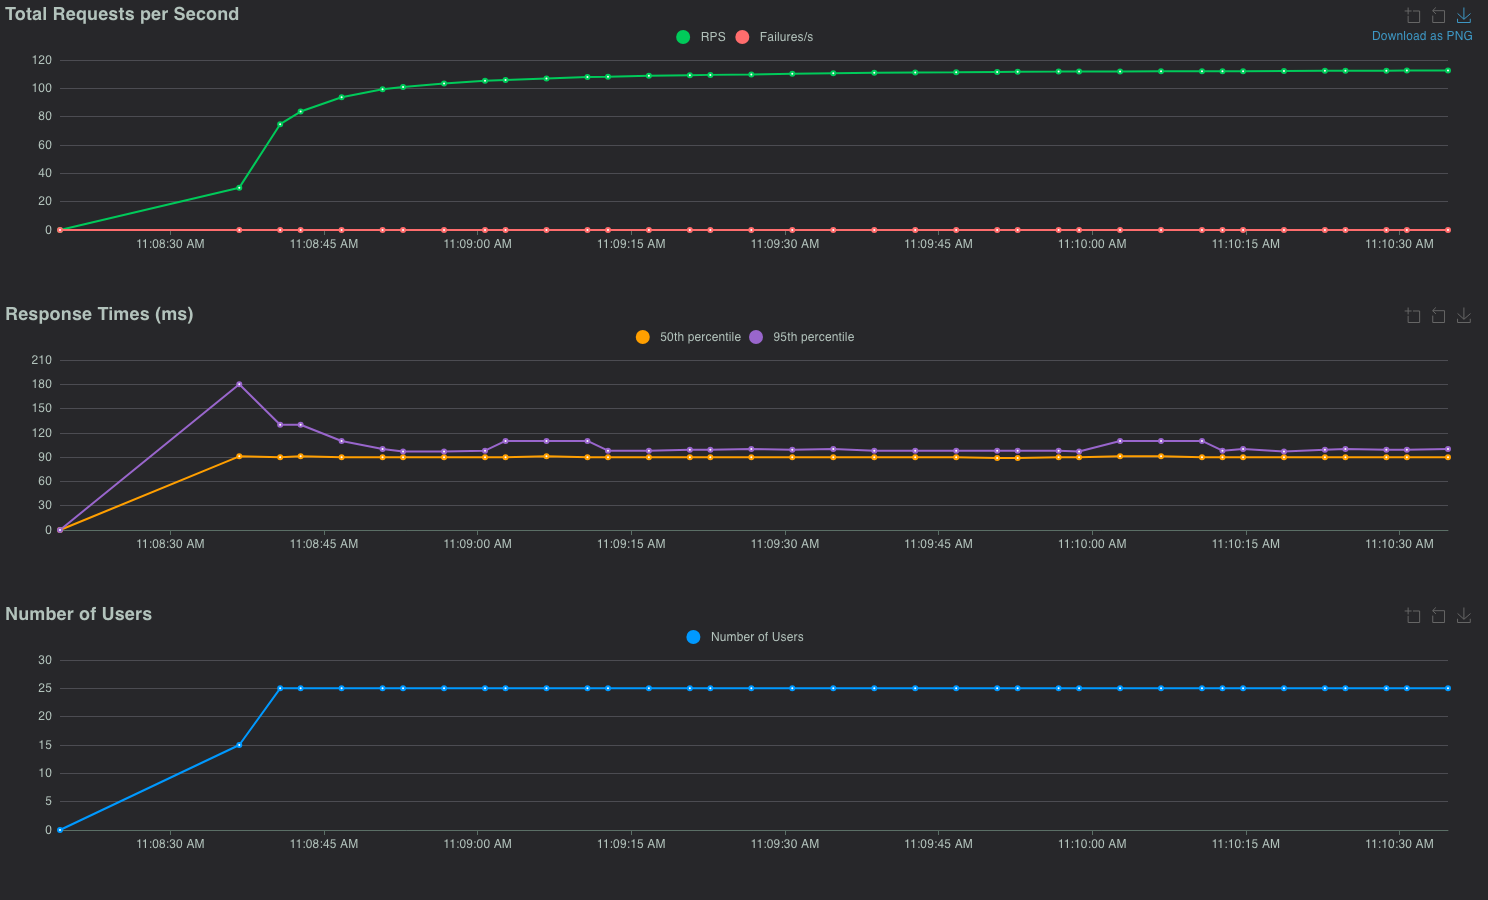
\includegraphics[width=0.95\textwidth]{screenshots/locust-hot-25u-charts.png}
\caption{Experiment~3 --- Locust Charts tab during a 25-user hot-account run.}
\label{fig:locust-hot-25-charts}
\end{figure}

\begin{figure}[H]
\centering
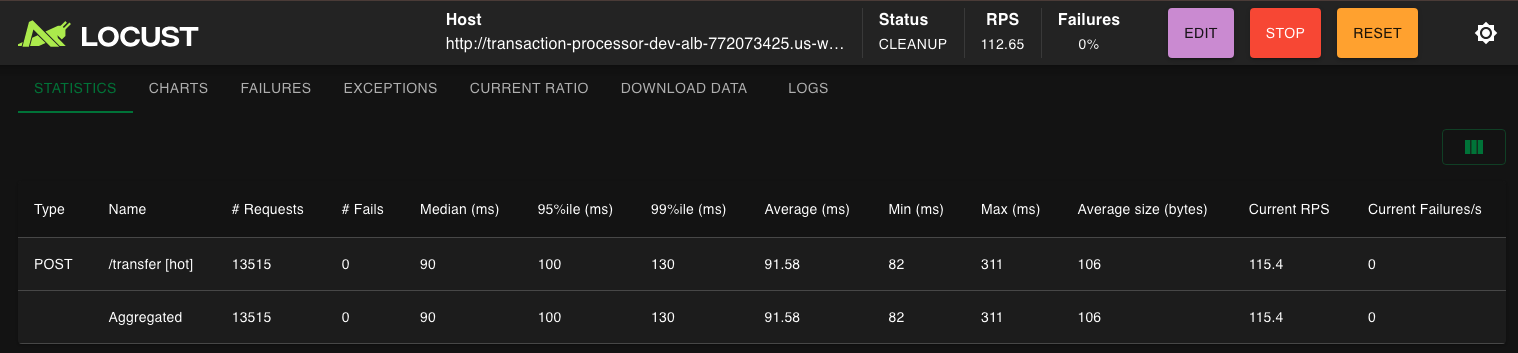
\includegraphics[width=0.95\textwidth]{screenshots/locust-hot-25u-stats.png}
\caption{Experiment~3 --- Locust Statistics tab for the same run.}
\label{fig:locust-hot-25-stats}
\end{figure}

\begin{figure}[H]
\centering
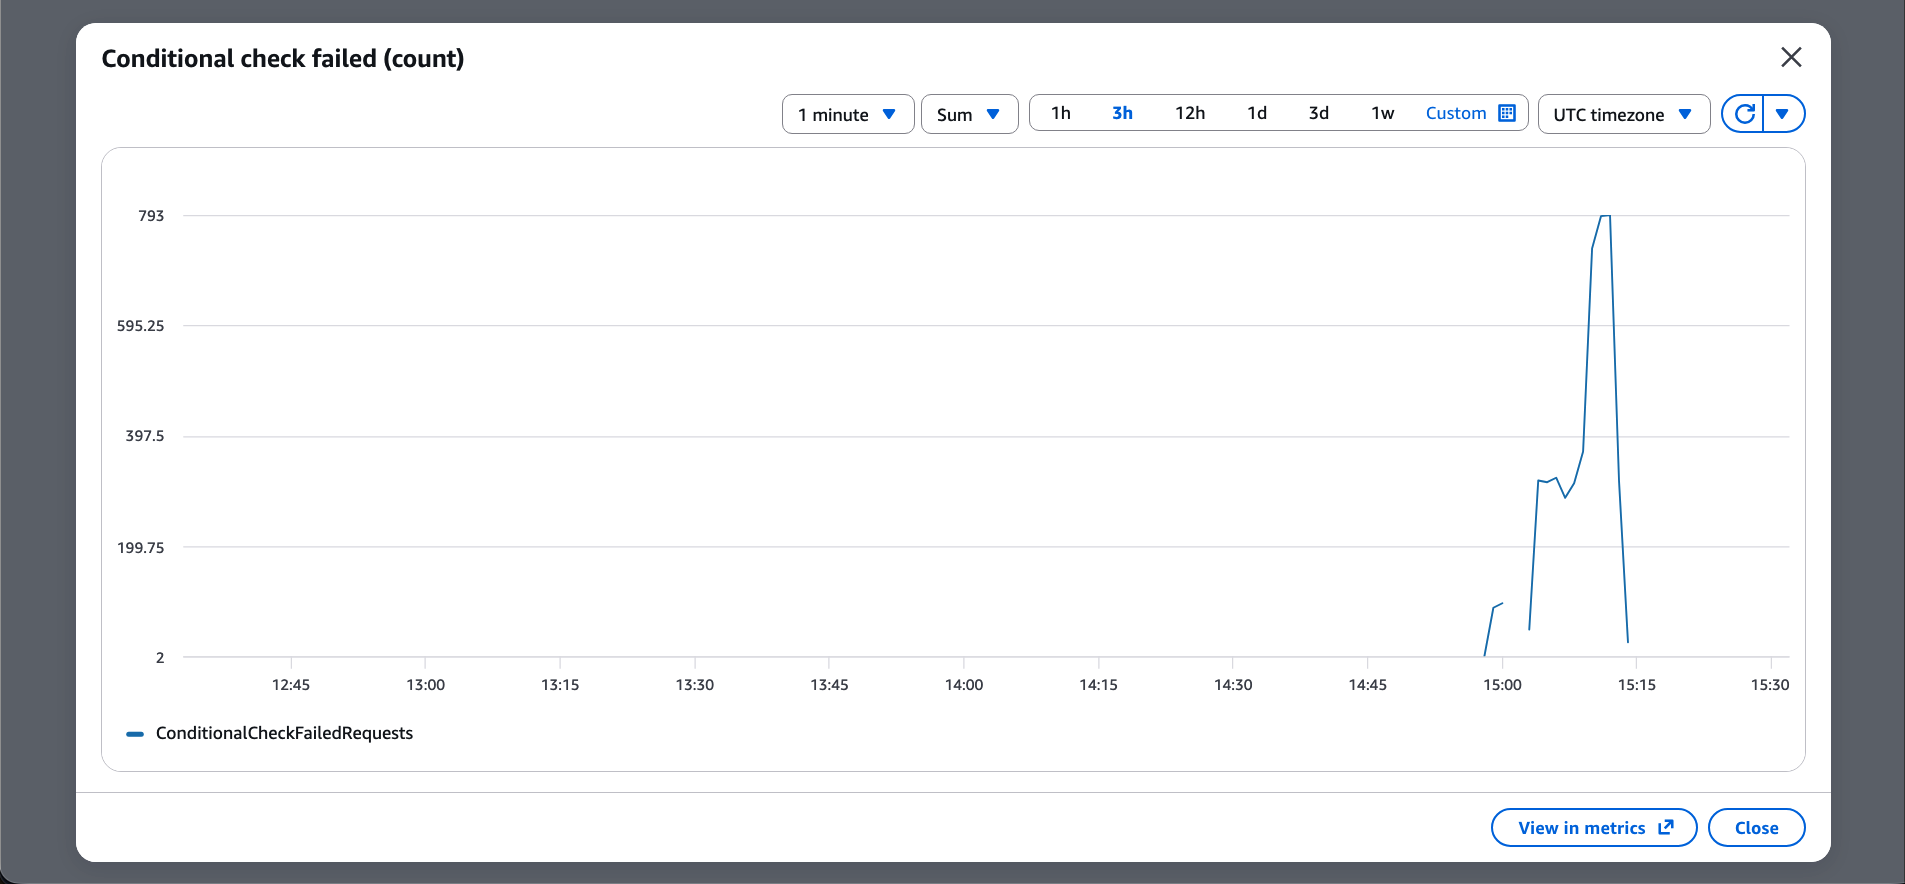
\includegraphics[width=0.95\textwidth]{screenshots/aws-dynamodb-conditional-fails.png}
\caption{DynamoDB \texttt{ConditionalCheckFailedRequests} graph across the Experiment~3 sweep. Optimistic traffic shows a steady rate of conditional-check failures (the version-mismatch retries); pessimistic traffic shows near-zero.}
\label{fig:ddb-cond-fails}
\end{figure}

%==============================================================
\section{Experiment~4 --- Horizontal Scaling}
%==============================================================

\subsection{Objective}
Hold the workload fixed, sweep the number of API and worker replicas through \{1, 2, 4\}, and measure how throughput and latency respond. This experiment tests whether the architecture actually scales horizontally or whether some hidden serialization point (database partition, ALB, queue depth) kicks in before we double replicas.

\subsection{Harness}
I wrote \texttt{scripts/scale\_experiment.sh}. Per replica pair it:
\begin{enumerate}[leftmargin=*, itemsep=0.2em]
    \item Runs \texttt{terraform apply} with \texttt{api\_desired\_count} and \texttt{worker\_desired\_count} set to the sweep values.
    \item Waits for both ECS services to stabilize.
    \item Purges SQS, sleeps past the visibility timeout, reseeds.
    \item Runs a 3-minute Locust \texttt{TransferUser} workload at 100 virtual users against the ALB.
    \item Waits for the queue to fully drain (up to 10~minutes), snapshots CloudWatch counters, verifies balances.
\end{enumerate}

\subsection{Results}

\begin{table}[H]
\centering
\caption{Experiment~4 results. \texttt{TransferUser}, 100 virtual users, 3-minute runs, optimistic mode.}
\label{tab:exp4}
\begin{tabular}{rrrrrr}
\toprule
API : Worker & Requests & Failures & Avg ms & p95 ms & Req/s \\
\midrule
1 : 1 & 15{,}176 & 0 & 850.78 & 1{,}600 & 84.53 \\
2 : 2 & 44{,}206 & 0 & 94.08  & 120    & 246.37 \\
4 : 4 & 44{,}372 & 0 & 92.79  & 110    & 247.35 \\
\bottomrule
\end{tabular}
\end{table}

\begin{figure}[H]
\centering
\begin{subfigure}[b]{0.48\textwidth}
    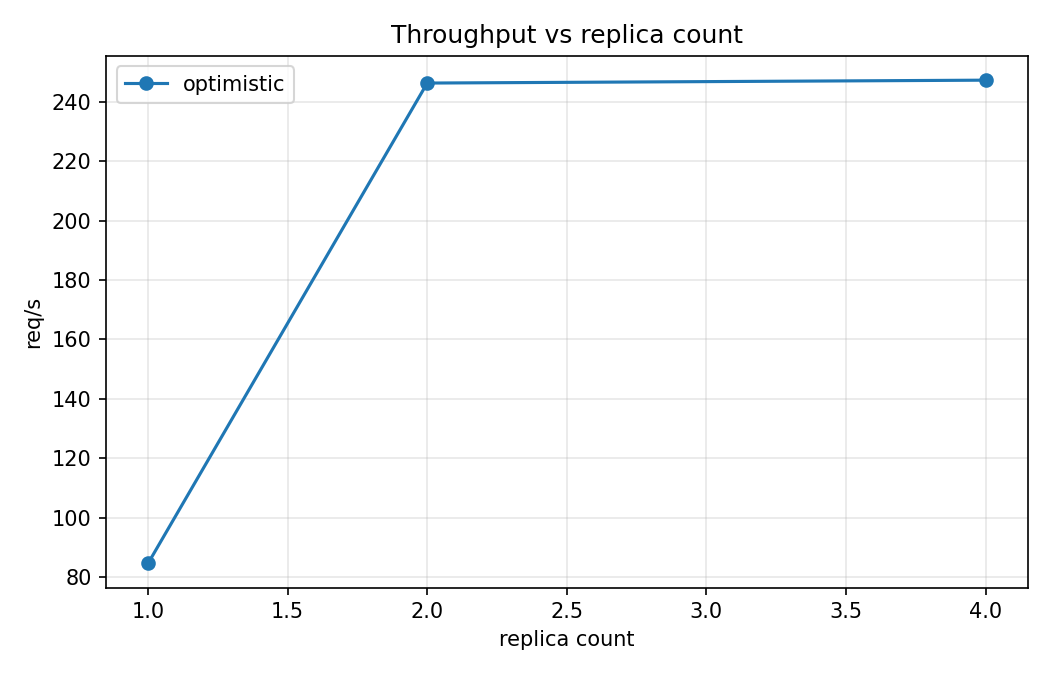
\includegraphics[width=\textwidth]{experiments/20260418-215633/scaling_throughput.png}
    \caption{Throughput vs. replica count.}
\end{subfigure}
\hfill
\begin{subfigure}[b]{0.48\textwidth}
    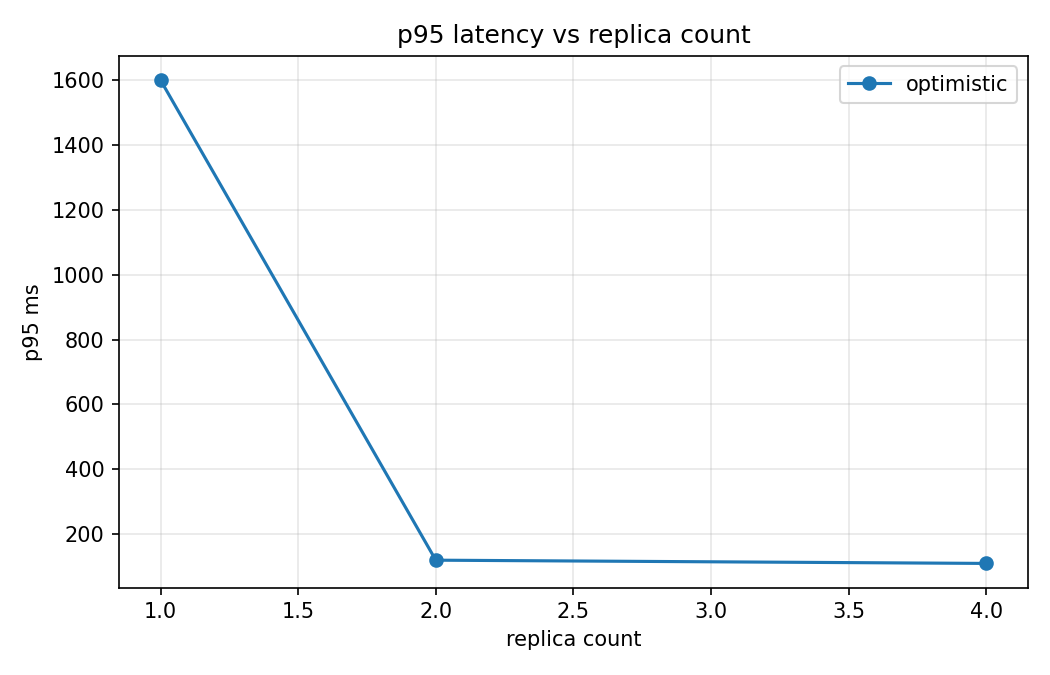
\includegraphics[width=\textwidth]{experiments/20260418-215633/scaling_p95.png}
    \caption{p95 latency vs. replica count.}
\end{subfigure}
\caption{Horizontal scaling curves for throughput and p95 latency.}
\label{fig:exp4}
\end{figure}

\subsection{Discussion}

Two distinct regimes emerged.

\textbf{1 $\rightarrow$ 2 replicas: near-ideal scaling.} Throughput jumped from 84.5 to 246.4~req/s, a factor of 2.9. Average latency collapsed from 850~ms to 94~ms (a 9$\times$ improvement) and p95 from 1{,}600~ms to 120~ms (a 13$\times$ improvement). A single worker at 100 virtual users was clearly saturated: messages queued up faster than one worker could drain them, pushing both queue depth and end-to-end latency up sharply.

\textbf{2 $\rightarrow$ 4 replicas: diminishing returns.} Throughput stayed flat at 247~req/s. p95 barely moved (120~ms $\rightarrow$ 110~ms). At this point the bottleneck is no longer the worker fleet. The three plausible culprits are (a) the Locust load generator itself at 100 users is throttled by its own think time, (b) the ALB target group is distributing all traffic but no more clients are driving it, or (c) DynamoDB's per-partition throughput is the ceiling now. Distinguishing among those would require a separate experiment with a larger Locust user pool, which was out of scope for this submission.

Balance correctness held for every configuration, which matters more than the raw numbers: doubling replicas did not expose any new race condition or lost update.

Figures~\ref{fig:locust-transfer-100-charts} and~\ref{fig:locust-transfer-100-stats} show the Locust-side view of the 100-user \texttt{TransferUser} workload that was held constant through the sweep; Figure~\ref{fig:sqs-monitoring} is the SQS Monitoring tab covering the full experiment --- message send, receive, and delete rates all rise and fall together as each replica-count iteration starts and finishes.

\begin{figure}[H]
\centering
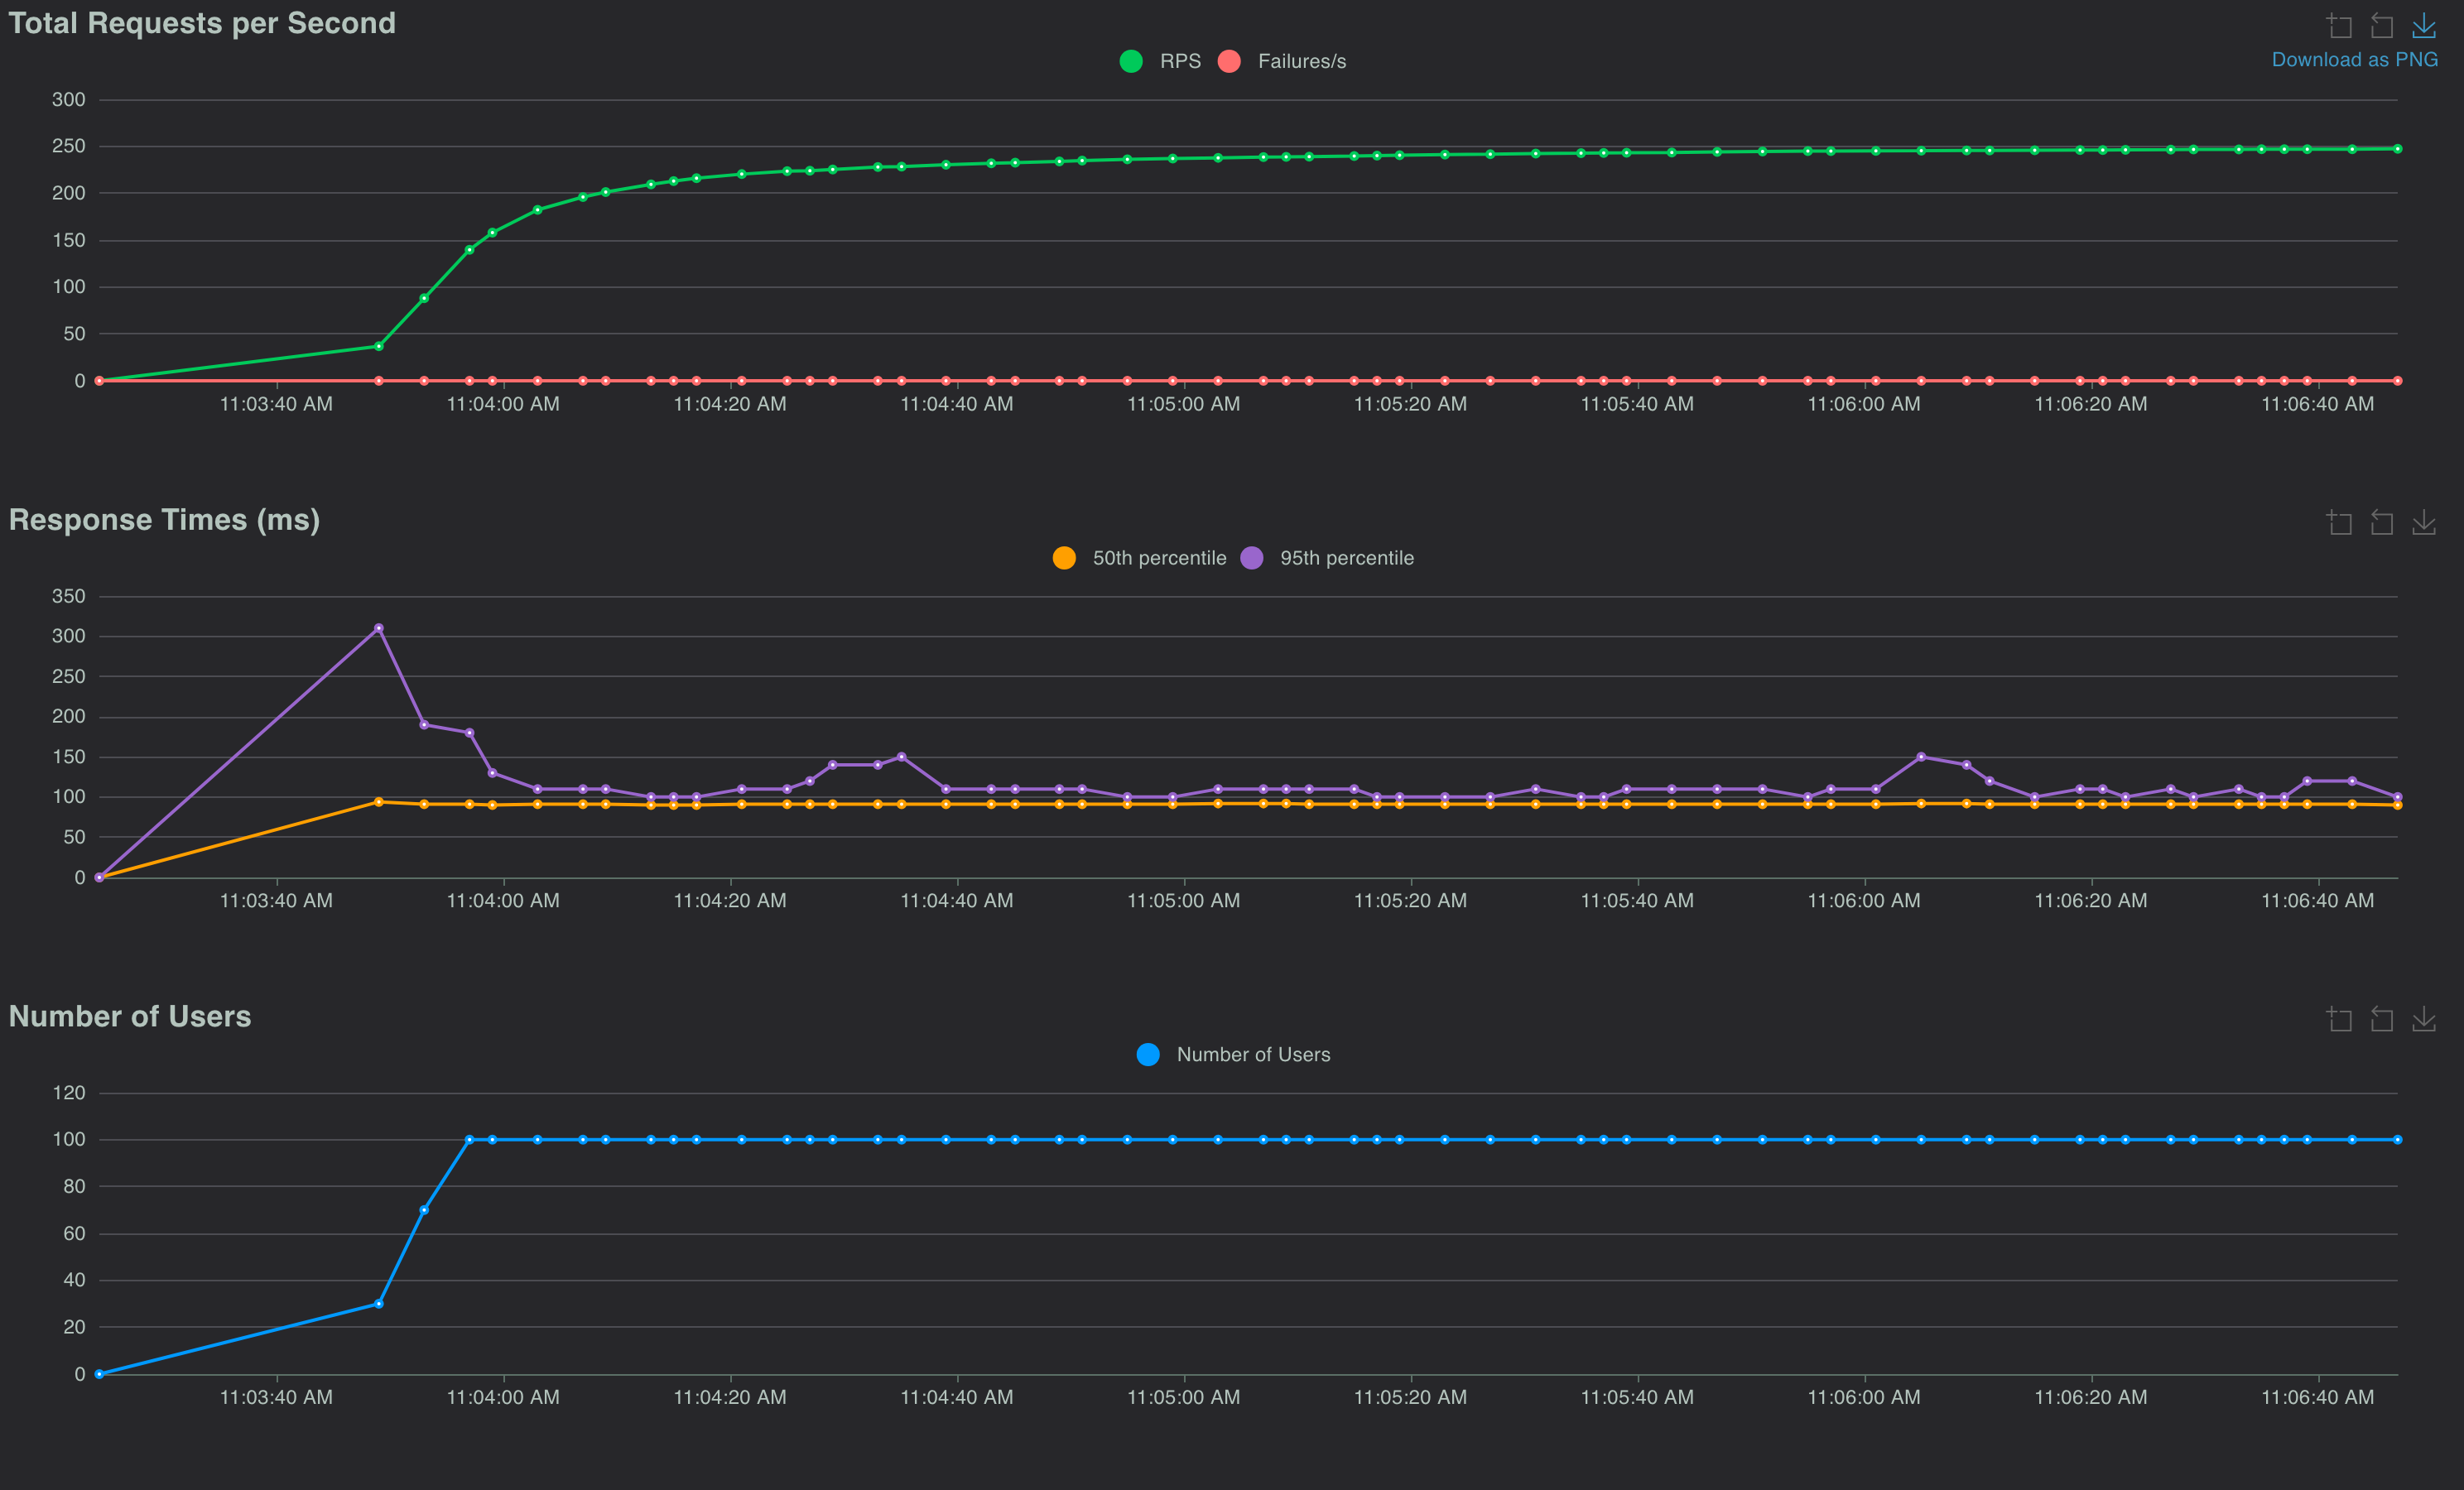
\includegraphics[width=0.95\textwidth]{screenshots/locust-transfer-100u-charts.png}
\caption{Experiment~4 --- Locust Charts tab at 100 \texttt{TransferUser} users.}
\label{fig:locust-transfer-100-charts}
\end{figure}

\begin{figure}[H]
\centering
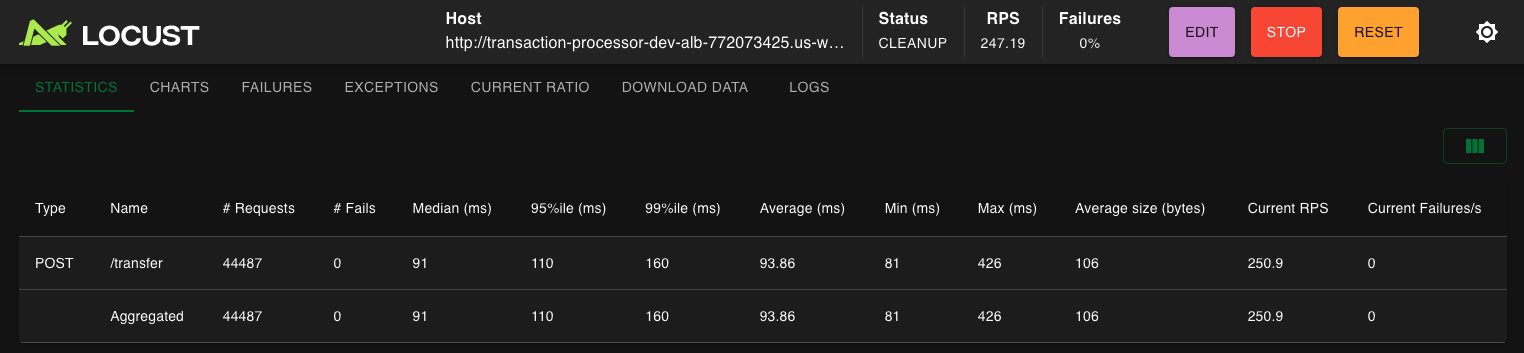
\includegraphics[width=0.95\textwidth]{screenshots/locust-transfer-100u-stats.png}
\caption{Experiment~4 --- Locust Statistics tab for the 100-user run.}
\label{fig:locust-transfer-100-stats}
\end{figure}

\begin{figure}[H]
\centering
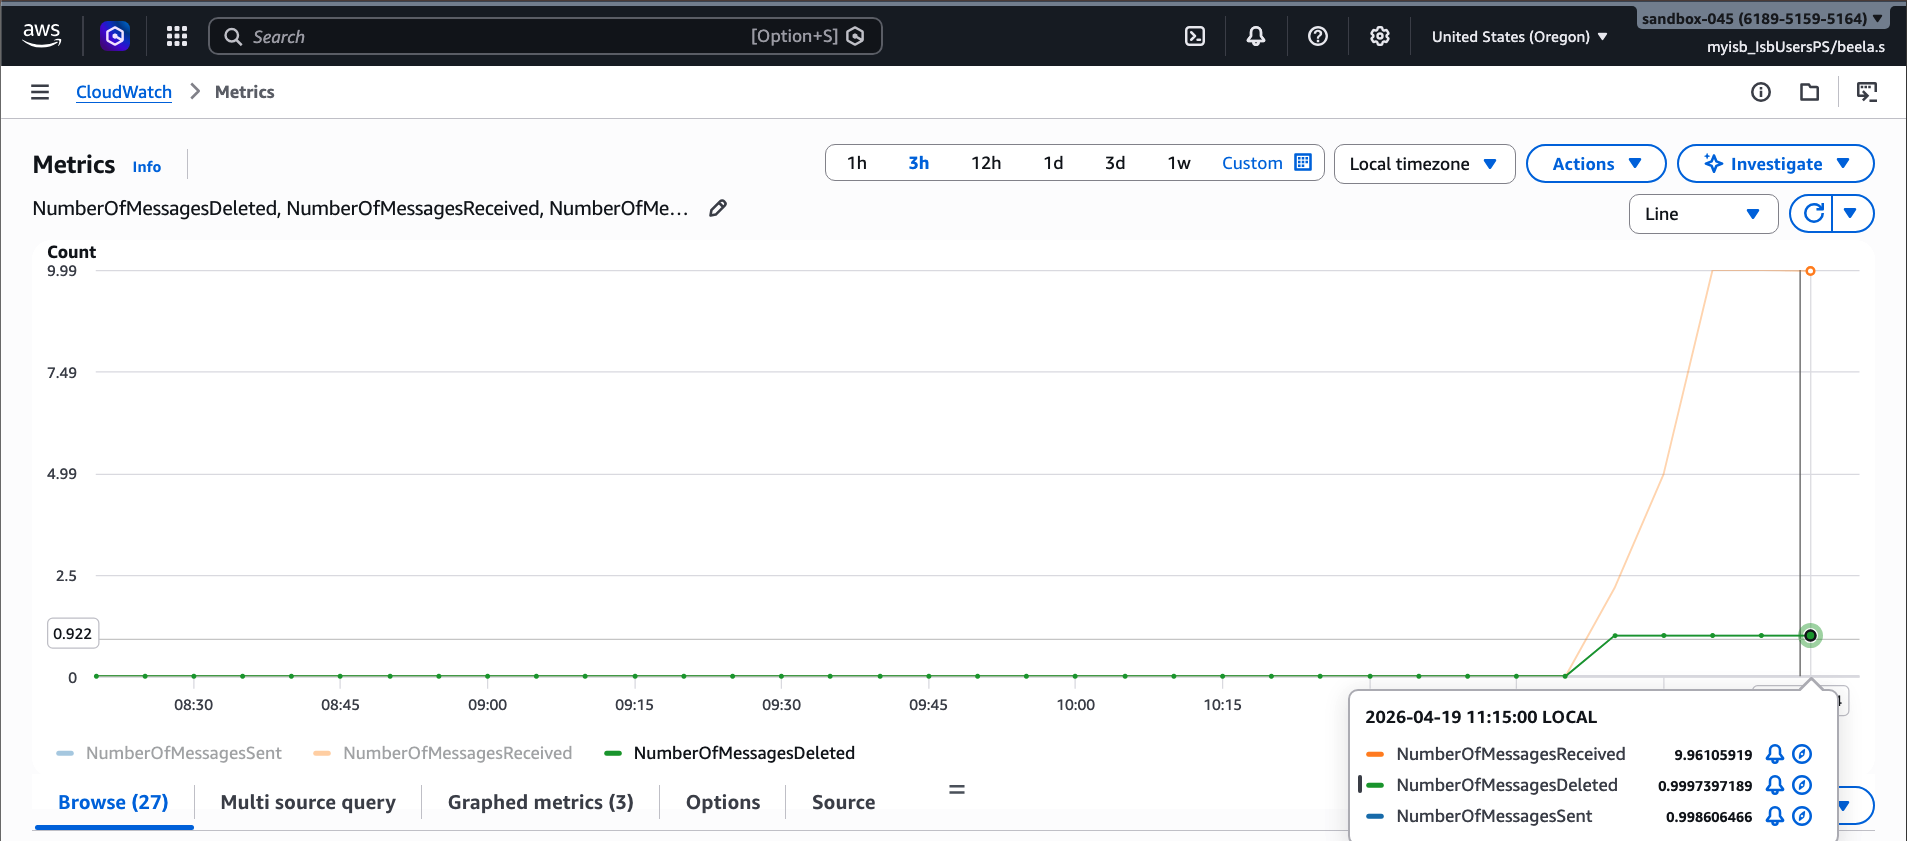
\includegraphics[width=0.95\textwidth]{screenshots/aws-sqs-monitoring.png}
\caption{SQS Monitoring tab spanning the Experiment~4 sweep. Each plateau is one replica-count iteration; the drops between them are the inter-run purge + drain windows.}
\label{fig:sqs-monitoring}
\end{figure}

%==============================================================
\section{Data Analysis and Chart Generation}
%==============================================================

The charts in Sections on Experiments~3 and~4 are produced by \texttt{scripts/render\_charts.py}, a matplotlib-based renderer I wrote. The script walks an experiments directory, reads each run's \texttt{.meta.json} (for mode, user count, and replica count labels), the Locust \texttt{\_stats.csv} (for throughput and latency), and optionally a \texttt{.metrics.json} snapshot scraped from CloudWatch (for conflict and retry rates). It emits PNGs at publication resolution:

\begin{itemize}[leftmargin=*, itemsep=0.2em]
    \item \texttt{throughput.png} and \texttt{p95\_latency.png} --- one bar per run.
    \item \texttt{conflict\_rate.png} and \texttt{retry\_rate.png} --- derived from the worker counters \texttt{transfer\_attempts\_total}, \texttt{transfer\_success\_total}, and \texttt{transfer\_conflicts\_total} per mode.
    \item \texttt{scaling\_throughput.png} and \texttt{scaling\_p95.png} --- line charts of the scaling experiment, one line per mode when a sweep covers multiple modes.
\end{itemize}

The chart generator reads from the per-experiment directory structure the sweep scripts produce, so re-running any experiment re-derives its charts without manual intervention. A \texttt{make charts DIR=load-tests/experiments/<stamp>} target wraps the Python call so the charts can be regenerated against any past run.

The metrics themselves come from the worker service: I added a small \texttt{metrics} package (\texttt{worker-svc/metrics/}) that exposes atomically incremented counters and serves them in Prometheus exposition format on port 9090. The worker also emits a structured JSON \texttt{METRICS} log line every 30~seconds so the experiment scripts can scrape cumulative values from CloudWatch Logs without needing direct network reachability to the ECS tasks. This is the glue that allows the chart pipeline to compute conflict and retry rates against a cloud deployment where the worker tasks have no inbound ingress.

Figure~\ref{fig:cw-worker} shows the CloudWatch log stream for the worker service during an experiment; the \texttt{METRICS} JSON lines are visible and match the schema the chart generator consumes.

\begin{figure}[H]
\centering
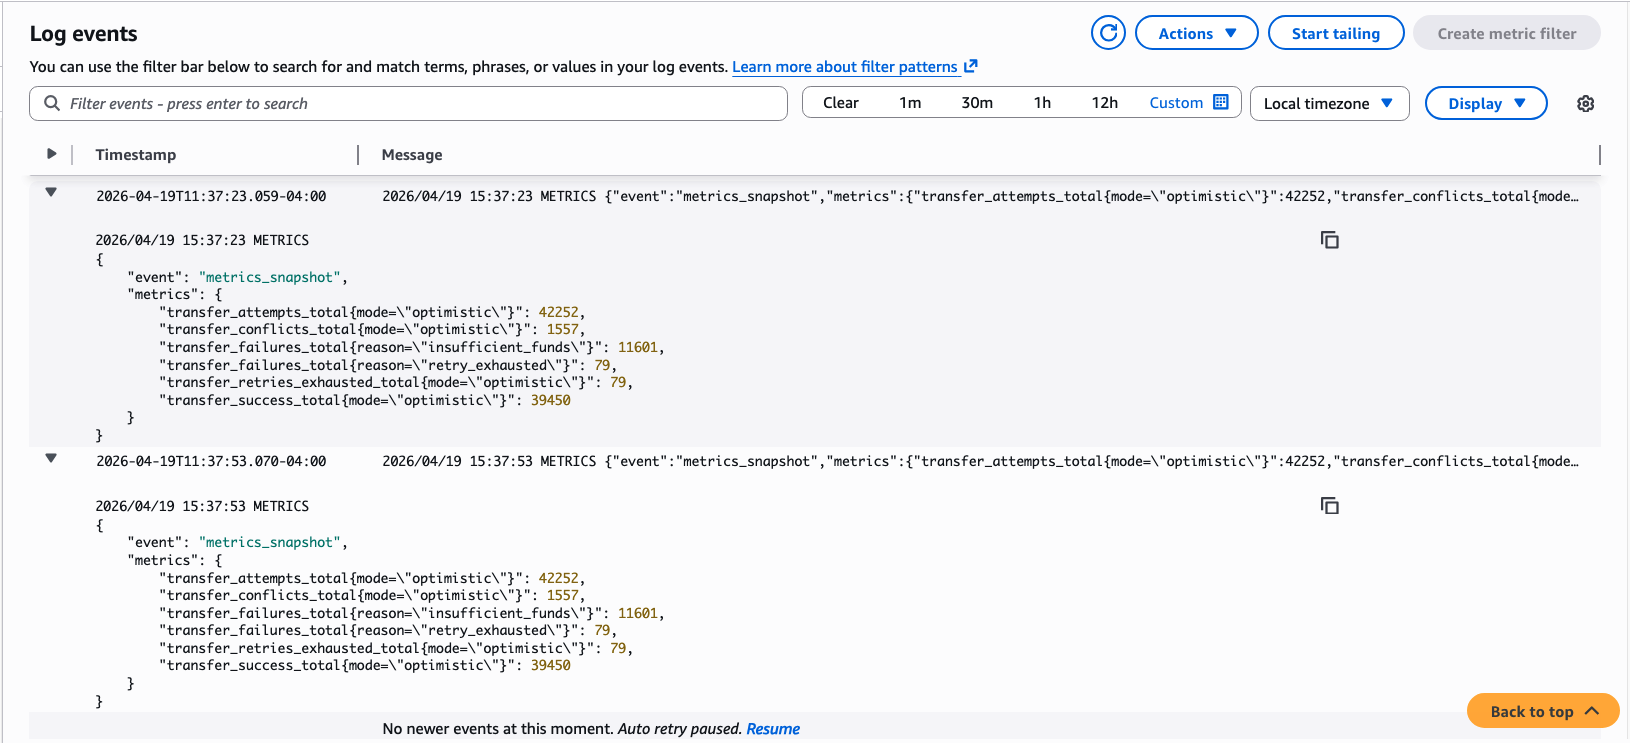
\includegraphics[width=0.95\textwidth]{screenshots/aws-cloudwatch-worker-logs.png}
\caption{Worker CloudWatch log stream with periodic \texttt{METRICS} JSON snapshots. Each snapshot contains cumulative values for every counter defined in Appendix C.}
\label{fig:cw-worker}
\end{figure}

%==============================================================
\section{Obstacles Encountered and Resolutions}
\label{sec:obstacles}
%==============================================================

Several non-trivial problems came up while bringing up and running the experiments. I list the ones that took real engineering work to diagnose and resolve.

\subsection{Cross-platform image builds}

The first attempt at deploying to Fargate failed with:

\begin{lstlisting}
CannotPullContainerError: image Manifest does not contain descriptor matching platform 'linux/amd64'
\end{lstlisting}

My laptop is Apple Silicon, so a plain \texttt{docker build} produces ARM64 images. Fargate's default runtime is \texttt{linux/amd64}. I switched \texttt{scripts/push\_images.sh} to use \texttt{docker buildx} with an explicit \texttt{--platform linux/amd64}. After the change, ECS task startup went from permanent failure to healthy in about 90 seconds.

\subsection{No default VPC in the chosen region}

Terraform's \texttt{data "aws\_vpc" "default"} lookup failed with \texttt{no matching EC2 VPC found} in \texttt{us-west-2}. The account had never had a default VPC created in that region. Running

\begin{lstlisting}
aws ec2 create-default-vpc --region us-west-2
\end{lstlisting}

once was enough to unblock every subsequent \texttt{terraform apply}.

\subsection{Shell-quoting on multiline IAM JSON}

My first attempts at creating the IAM role from the shell kept being mangled by zsh's brace expansion:

\begin{lstlisting}
aws: error: the following arguments are required: --assume-role-policy-document
zsh: command not found: --assume-role-policy-document
\end{lstlisting}

I moved the trust policy into a committed file (\texttt{infra/labrole-trust.json}) and wrote \texttt{scripts/bootstrap\_labrole.sh} to create the role and attach the four managed policies (\texttt{AmazonECSTaskExecutionRolePolicy}, \texttt{AmazonDynamoDBFullAccess}, \texttt{AmazonSQSFullAccess}, \texttt{CloudWatchLogsFullAccess}). The script is idempotent so re-running it is safe.

\subsection{macOS \texttt{date} has no millisecond format}

Both sweep scripts originally computed a CloudWatch ``since'' timestamp with \texttt{\$(date +\%s\%3N)}. On macOS that produced literal output like \texttt{17765569773N}, which then failed arithmetic:

\begin{lstlisting}
./scripts/compare_locking_modes.sh: line 114: 17765569773N: value too great for base
\end{lstlisting}

I replaced both occurrences with \texttt{python3 -c 'import time; print(int(time.time()*1000))'}, which is portable across macOS and Linux.

\subsection{Queue drainage between iterations}

Early scale-experiment runs showed small transient balance mismatches (on the order of \$79--\$89) because the balance verification ran before all in-flight transfers had committed. The total was always correct moments later.

I did two things:
\begin{enumerate}[leftmargin=*, itemsep=0.2em]
    \item Added a drain loop that waits until both \texttt{ApproximateNumberOfMessages} and \texttt{ApproximateNumberOfMessagesNotVisible} reach zero, plus a 15-second settle buffer, before invoking the balance verifier.
    \item Switched the scan in the verifier to \texttt{ConsistentRead=True} so pagination doesn't see a mix of old and new item versions during active writes.
\end{enumerate}

After both changes, every experiment reports either a zero difference or a difference consistent with float64 rounding (on the order of $10^{-12}$).

\subsection{Reseed racing with in-flight workers}

When a sweep finishes one iteration and starts the next, the reseed step ran into \texttt{TransactionConflictException} because in-flight worker transactions held a short transactional lock on the items being overwritten:

\begin{lstlisting}
TransactionConflictException: Transaction is ongoing for the item
\end{lstlisting}

I added exponential-backoff retry handling to \texttt{scripts/seed\_accounts.go} specifically for this error code (up to 8 attempts, capped at 3~s between tries), and I added an explicit SQS purge plus 65-second drain before reseed in both sweep scripts. Together these changes made the between-iteration reset deterministic.

\subsection{Locust environment hygiene}

The load-test venv on my laptop had a stale \texttt{zope.event} dependency that broke Locust import. A clean-slate venv

\begin{lstlisting}
python3 -m venv /tmp/locust-venv
/tmp/locust-venv/bin/pip install --upgrade pip locust boto3
\end{lstlisting}

solved it. I also added \texttt{boto3} to the venv so \texttt{verify\_balances.py} runs under the same interpreter as Locust, which avoids the Makefile picking the wrong Python.

%==============================================================
\section{Demo Preparation}
%==============================================================

The demo is scripted around the four experiments, in the same order they run in production:

\begin{enumerate}[leftmargin=*, itemsep=0.2em]
    \item \texttt{make preflight} --- show that the caller is an SSO session but that \texttt{LabRole} exists and is assumable by ECS. This establishes the IAM story on camera.
    \item \texttt{make cloud-smoke} --- end-to-end transfer via the ALB in under 10~seconds.
    \item \texttt{make cloud-test-load-hot} (partial, one minute) --- Experiment~1 in miniature, with live Locust throughput on stdout.
    \item \texttt{make cloud-compare-locking} against a pre-run artifact directory --- explain Experiment~3's charts side by side.
    \item \texttt{make scale-experiment} artifacts --- walk through the scaling curve and the saturation story.
    \item \texttt{make tf-destroy} --- tear down everything on camera to close the loop.
\end{enumerate}

All of these targets are preflight-gated and read their inputs from Terraform outputs, so the demo is safe to run live without any environment-specific shell state.

%==============================================================
\section{Conclusion}
%==============================================================

My half of this project covers the outward-facing and stress-testing surface of the system. I designed and agreed the architecture, scaffolded the two services, wired the API to SQS, packaged both services for AWS Fargate, wrote the Locust harness, and ran three of the four experiments end-to-end on real AWS infrastructure. The correctness invariant held under every workload we threw at it: the sum of balances equalled the seeded total, to within float-rounding tolerance, after every run. The performance envelope is well characterized:

\begin{itemize}[leftmargin=*, itemsep=0.2em]
    \item Hot-account contention at 50 users: 115~req/s, p95 530~ms, zero failed transfers.
    \item Optimistic and pessimistic locking tie on throughput at our contention levels; pessimistic wins p95 at low contention by avoiding retry backoff.
    \item Doubling replicas from 1 to 2 gives near-ideal scaling ($2.9\times$ throughput, $13\times$ better p95). Scaling past 2 hits a load-generator or partition-throughput ceiling that future work would need a larger client pool to explore.
\end{itemize}

The work also demonstrates a practical cloud-deployment discipline: every \texttt{make} target is gated by a \texttt{LabRole} preflight, Terraform refuses to plan or apply if the role isn't properly wired, and no IAM resources are ever created by the stack. This means the experiments are reproducible on any AWS account that has a \texttt{LabRole}-shaped role, without ever needing elevated permissions at apply time.

%==============================================================
\appendix
\section{Artifact Index}
%==============================================================

\begin{itemize}[leftmargin=*, itemsep=0.2em]
    \item Repository root: \texttt{transaction-processor/}
    \item Architecture: \texttt{arch.md} (source), Figure~\ref{fig:arch} (rendered)
    \item API service: \texttt{api-svc/}
    \item Worker service: \texttt{worker-svc/}
    \item Terraform stack: \texttt{infra/}
    \item Load testing: \texttt{load-tests/locustfile.py}
    \item Experiment runners: \texttt{scripts/compare\_locking\_modes.sh}, \texttt{scripts/scale\_experiment.sh}
    \item Chart generator: \texttt{scripts/render\_charts.py}
    \item Preflight: \texttt{scripts/preflight\_labrole.sh}
    \item Experiment artifacts: \texttt{load-tests/experiments/20260418-200951/} (Experiment~3), \texttt{load-tests/experiments/20260418-215633/} (Experiment~4)
    \item Experiment~1 aggregate: \texttt{load-tests/results-hot\_stats.csv}
\end{itemize}

\section{Makefile Target Reference}

\begin{lstlisting}
make preflight              # assert LabRole exists + ECS-assumable
make tf-init / tf-apply     # terraform bringup (preflight-gated)
make push-images            # cross-build + push amd64 images to ECR
make cloud-seed             # seed 101 accounts into cloud DynamoDB
make cloud-smoke            # end-to-end transfer via ALB
make cloud-test-load        # mixed-workload Locust run
make cloud-test-load-hot    # Experiment 1 hot-account storm
make cloud-compare-locking  # Experiment 3 sweep
make scale-experiment       # Experiment 4 sweep
make charts DIR=...         # re-render PNGs from an experiments directory
make tf-destroy             # tear down the cloud stack
\end{lstlisting}

\section{Key Counter Definitions}

The worker exposes six cumulative counters used across the experiments:

\begin{itemize}[leftmargin=*, itemsep=0.2em]
    \item \texttt{transfer\_attempts\_total\{mode\}} --- every call into the transfer loop.
    \item \texttt{transfer\_success\_total\{mode\}} --- every successful commit.
    \item \texttt{transfer\_conflicts\_total\{mode\}} --- every retryable concurrency conflict (optimistic: version mismatch; pessimistic: cancelled transaction).
    \item \texttt{transfer\_retries\_exhausted\_total\{mode\}} --- transfers that gave up after the three-attempt budget.
    \item \texttt{transfer\_failures\_total\{reason\}} --- terminal \texttt{FAILED} outcomes tagged with reason (insufficient funds, missing account, retry exhausted).
    \item \texttt{transfer\_lock\_acquire\_failed\_total\{mode\}} --- pessimistic lease acquisition failures.
\end{itemize}

\end{document}
